%%%%%%%
% vr-thesis-template.tex
%%%%%%%

% Import preamble settings
% Document class
\documentclass[fontsize=12pt, paper=a4, headinclude, twoside=false, parskip=half+, pagesize=auto, numbers=noenddot, plainheadsepline, open=right, toc=listof]{scrreprt}
\usepackage[standardsections]{scrhack}

% PDF compression
\pdfminorversion=5
\pdfobjcompresslevel=1

% General
%\usepackage[automark]{scrpage2}          % Header and Footer
\usepackage[automark]{scrlayer-scrpage}  % Header and Footer
\usepackage{amsmath, marvosym}           % Math libraries
\usepackage[utf8]{inputenc}              % UTF8-Encoding
\usepackage{amsthm}
\usepackage[bottom]{footmisc}
\usepackage[acronym]{glossaries}

% Font
\usepackage{mathpazo}                    % Palatino for math
\usepackage{setspace}                    % Line space
\onehalfspacing                          % Line space 1.5
\setkomafont{chapter}{\Huge\rmfamily}    
\setkomafont{section}{\Large\rmfamily}
\setkomafont{subsection}{\large\rmfamily}
\setkomafont{subsubsection}{\large\rmfamily}
\setkomafont{chapterentry}{\large\rmfamily}
\setkomafont{descriptionlabel}{\bfseries\rmfamily}
\setkomafont{captionlabel}{\small\bfseries}
\setkomafont{caption}{\small}
\usepackage{amssymb}
\usepackage{tcolorbox}

% Language: English
\usepackage[british]{babel}

% PDF-Output
\usepackage[british, colorlinks=false, linkcolor=black]{hyperref}
\usepackage[final]{microtype}
\usepackage{url}
\usepackage{pdflscape}

% Tables
\usepackage{multirow}
\usepackage{multicol}
\usepackage{tabularx}
\usepackage{array}
\usepackage{float}
\usepackage{varwidth}
\usepackage{verbatimbox}

% Images
\usepackage{graphicx}
\usepackage{color}
\graphicspath{{images/}}
\DeclareGraphicsExtensions{.pdf,.png,.jpg}
\usepackage{subfigure}
\newcommand{\subfigureautorefname}{\figurename}
\usepackage[all]{hypcap}
\setcapindent{0em}
\setcapwidth[c]{0.9\textwidth}
\setlength{\abovecaptionskip}{0.2cm}

% Source code
\usepackage{listings}

\definecolor{mygreen}{rgb}{0,0.6,0}
\definecolor{mygray}{rgb}{0.5,0.5,0.5}
\definecolor{mymauve}{rgb}{0.58,0,0.82}

\lstset{ %
  backgroundcolor=\color{white},   % choose the background color
  basicstyle=\scriptsize\ttfamily,        % size of fonts used for the code
  breaklines=tduringrue,                 % automatic line breaking only at whitespace
  captionpos=b,                    % sets the caption-position to bottom
  commentstyle=\color{mygreen},    % comment style
  escapeinside={\%*}{*)},          % if you want to add LaTeX within your code
  keywordstyle=\color{blue},       % keyword style
  stringstyle=\color{mymauve},     % string literal style
  frame=single
}

% Quotes
\usepackage{epigraph}
\setlength\epigraphwidth{10cm}
\setlength\epigraphrule{0pt}
\usepackage{etoolbox}
\makeatletter
\patchcmd{\epigraph}{\@epitext{#1}}{\itshape\@epitext{#1}}{}{}
\makeatother

% Title style
\usepackage{titlesec, blindtext}
\definecolor{gray75}{gray}{0.75}
\newcommand{\hsp}{\hspace{20pt}}
\titleformat{\chapter}[block]{\Huge\bfseries}{\thechapter\hsp\textcolor{gray75}{$\vert$}\hsp}{0pt}{\Huge\bfseries}

% Title spacing
\titlespacing*{\chapter}{0pt}{0pt}{20pt}


% left-aligned footnotes
\deffootnote{1.5em}{1em}{\makebox[1.5em][l]{\thefootnotemark}}

\typearea{14}
\makeatletter
\newcommand{\saved@equation}{}
\let\saved@equation\equation
\def\equation{\@hyper@itemfalse\saved@equation}
\makeatother

% cites with text in them
\makeatletter
\let\cite\relax
\DeclareRobustCommand{\cite}{%
  \let\new@cite@pre\@gobble
  \@ifnextchar[\new@cite{\@citex[]}}
\def\new@cite[#1]{\@ifnextchar[{\new@citea{#1}}{\@citex[#1]}}
\def\new@citea#1{\def\new@cite@pre{#1}\@citex}
\def\@cite#1#2{[{\new@cite@pre\space#1\if\relax\detokenize{#2}\relax\else, #2\fi}]}
\makeatother

% Hypothesis Counters
% Parameters of newtheoremstyle: ABOVESPACE, BELOWSPACE, BODYFONT, INDENT, HEADFONT, HEADPUNCT, HEADSPACE, CUSTOM-HEAD-SPEC

\newtheoremstyle{hypothesisstyle}  
  {\topsep}
  {0}
  {\normalfont}
  {0pt}
  {\bfseries}
  {:}
  {5pt plus 1pt minus 1pt}
  {\thmname{#1}\textsubscript{\thmnumber{#2}}}

\newtheoremstyle{shypothesisstyle}
  {\topsep}
  {0}
  {\small}
  {5pt}
  {\itshape\bfseries}
  {:}
  {5pt plus 1pt minus 1pt}
  {\thmname{#1}\textsubscript{\thmnumber{#2}}}

\theoremstyle{hypothesisstyle}
\newtheorem{hypothesis}{H}[]
\theoremstyle{shypothesisstyle}
\newtheorem{shypothesis}{H}[hypothesis]
\renewcommand*{\theshypothesis}{\arabic{hypothesis}\alph{shypothesis}}
\usepackage{cleveref}
\crefformat{hypothesis}{\textbf{H\textsubscript{#1}}}
\crefformat{shypothesis}{\textbf{\textit{H\textsubscript{#1}}}}
\newcommand{\hypref}[1]{\hyperref[#1]{\cref{#1}}}

% further commands
\newcommand{\todo}[1]{\colorbox{red}{\textbf{TODO:} #1}}
\newcommand{\degree}[1]{#1^{\circ}}

% acronyms 
\newacronym{vr}{VR}{Virtual Reality}
\newacronym{hmd}{HMD}{Head-Mounted Display}
\newacronym{ve}{VE}{Virtual Environments}

% buw title page
\makeatletter
\newcommand*{\studyprogramme}[1]{\def\@studyprogramme{#1}}
\newcommand*{\matnr}[1]{\def\@matnr{#1}}
\newcommand*{\birthdate}[1]{\def\@birthdate{#1}}
\newcommand*{\birthplace}[1]{\def\@birthplace{#1}}
\newcommand*{\firstref}[1]{\def\@firstref{#1}}
\newcommand*{\secondref}[1]{\def\@secondref{#1}}
\newcommand*{\submissiondate}[1]{\def\@submissiondate{#1}}

\def\maketitle
{%
\clearscrheadings
\clearscrplain

Bauhaus-Universität Weimar \\
Faculty of Media \\
Degree Programme \@studyprogramme

\vspace{30mm}

\begin{center}

\begin{huge}
\@title
\end{huge}\\ \vspace{0.25cm}
\begin{LARGE}
\@subtitle
\end{LARGE}


\vspace{13mm}
\begin{Large}
Master's Thesis
\end{Large}
\end{center}

\vspace{25mm}

\@author \hfill Matriculation number: \@matnr \\
born on \@birthdate{} in \@birthplace

\vspace{3.5cm}

\begin{tabular}{@{}ll}
{\textbf{First referee:}} & \@firstref \\
{\textbf{Second referee:}} & \@secondref \\
\end{tabular}

\vspace{1cm}
Submission date: \@submissiondate

\clearpage
}
\makeatother 

\begin{document}

% Roman numbering in the beginning
\pagenumbering{Roman}
\pagestyle{empty}


%%%%%%%
% Title page (appearance defined in preamble)
%%%%%%%

\studyprogramme{Human-Computer Interaction}
\title{Jumping for Guided Navigation in Immersive Virtual Environments}
%\subtitle{Optional Subtitle of the Thesis}
\author{Ramsha Saad Thaniana}
\matnr{121766}
\birthdate{07\textsuperscript{th} October 1996}
\birthplace{Karachi, Pakistan}
\firstref{Prof. Dr. Bernd Fröhlich}
\secondref{Junior-Prof. Dr. Jan Ehlers}
\submissiondate{08\textsuperscript{th} November 2021}

\maketitle

% Normal headers and footers for the remainder
\pagestyle{useheadings}

%%%%%%%
% Declaration of Authorship
%%%%%%%

\chapter*{Declaration of Authorship}
I hereby declare that I have written this thesis without the use of documents and aids other than those stated in the references, that I have mentioned all sources used and that I have cited them correctly according to established academic citation rules, and that the topic or parts of it are not already the object of any work or examination of another study programme.

\vspace{4cm}

Date \hspace{\fill} \makeatletter\@author\makeatother \\


%%%%%%%
% Abstract
%%%%%%%

\chapter*{Abstract}
\label{Abstract}
With the advance of Virtual Reality, there is a case to be made for narrative experiences such as tours and storytelling to be made virtual as well. This thesis presents a technique for automated guided jumping navigation in immersive virtual environments. The implementation of this technique includes how jumps will take place, pre-travel feedback and gesture control to pause, resume and make choices when needed. To investigate the benefits of this technique, this thesis presents a user study comparing automated guided jumping with free jumping using visual guidance. The results from conducting this study with 9 participants show that automated guided jumping provides similar path recall scores to free jumping. They also show that although free jumping gives lower discomfort scores, higher user comfort, lower task load scores and better comprehensibility of jumps, automated guided jumping still has good results for all these variables. Overall, the study shows that the technique has benefits and potential for further improvement in future work to create immersive environments that provide a narrative structure and require minimal user control.

%%%%%%%
% Table of contents
%%%%%%%

\tableofcontents

%%%%%%%
% Main content
%%%%%%%

%%%%%%%
% Introduction
%%%%%%%

\chapter{Introduction}
\pagenumbering{arabic}
%This is the introduction...
%
%\vspace{0.5cm}
%
%\begin{figure}[]
%  \centering
%  
\includegraphics[width=0.5\textwidth]{images/todo.png}
%  \caption{This is an example ToDo picture.}
%  \label{fig:todo}
%\end{figure}
\label{Chapter:Introduction}
Many navigation techniques exist for both Desktop and Immersive \acrfull{ve} that define how users moves around these \acrshort{ve}s. The goals of navigation are to move towards a target location and orientation to explore the environment. Navigation should facilitate way finding in the \acrshort{ve}, which means allowing the user to know where they are, where they will go next and how they will get there. This also means that the user should have a good perception of the \acrshort{ve} and path that they took. Navigation techniques have to ensure that there is minimal motion sickness, sufficient environmental awareness which means that while navigating the user knows where they are in an environment compared to where they were before and that it is easy to reach important places in the environment. Two common metaphors for navigation are steering and teleportation.

Steering navigation is a technique where there is continuous movement in a direction indicated either by gaze, pointing or use of a physical device. In some cases an additional action can be added to specify the velocity. With steering navigation spatial awareness is generally good but can cause motion sickness. Teleportation navigation is a target based metaphor for where the goal position is specified discretely by pointing or choosing a location and orientation to be moved towards. This form of navigation minimises motion sickness but results in less environmental awareness as compared to the steering metaphor. Some techniques try to reconcile these two metaphors to minimise motion sickness while still maintaining a good environmental awareness. One example is the jumping metaphor presented by Weissker et al. which \textit{'only allows to teleport to locations in the currently visible part of the scene'} which makes it a short range version of the teleportation metaphor~\cite{Weissker2018}. 

Navigation techniques can be active such that the user is controlling their own movement; passive such that the user is being automatically moved around the environment; or they can be a mix of active and passive. Navigation techniques can also provide the user with guidance regardless of whether this is active or passive. Guided navigation techniques such as the river analogy presented by Galyean, which guides \textit{'the user’s continuous and direct input within both space and time allowing a more narrative presentation'} and uses automatic steering for guided navigation allow for the addition of a narrative structure to a \acrshort{ve}~\cite{Galyean1995}. In this work we will explore guided navigation using the jumping metaphor instead of a steering one and investigate the benefits of an automatic approach over a user controlled one for a museum setting. 

This thesis will discuss work related to navigation techniques and guiding in \acrshort{ve}s on \acrfull{hmd}s in Chapter \ref{Chapter:Related Work}. Then in Chapter \ref{Chapter:Guided Jumping Motivation} it will look into the motivation and use cases for a technique that combines guiding with navigation for an automated guided navigation technique using jumping. Based on these motivations Chapter \ref{Chapter:Automated Guided Jumping} will look at the design and development of an automated guided navigation technique. To justify the benefits of this proposed technique in comparison to a technique with free jumping using visual guidance, a study design and procedure will be introduced in Chapter \ref{Chapter:Design and Procedure of the User Study}. Then Chapter \ref{Chapter:Evaluation of the User Study} will look at the results of this study. The thesis will then be concluded in Chapter \ref{Chapter:Conclusion and Future Work} which will summarize the results and propose some future work that can be done on the topic of automated guided jumping for navigation in \acrshort{ve}s.


%%%%%%%
% Related Work
%%%%%%%

\chapter{Related Work}
\pagenumbering{arabic}
\label{Chapter:Related Work}
As mentioned in \cref{Chapter:Introduction}, this thesis aims to investigate a technique for automated guided navigation using the jumping metaphor. To understand where the concept for this technique comes from, we will take a look at different navigation metaphors for \acrshort{hmd}s and see what the advantages of jumping navigation are. We will then see what the purpose of guiding in \acrshort{ve}s is and why it can be useful for navigation to be guided. Based on this, we will then show the motivation for bringing together jumping and guiding into one navigation technique. 

\section{Navigation}
\label{section RW: Navigation}

Navigation is the task of moving around and when it comes to \acrfull{3d} environments it is one of the most common actions that is carried out by users. According to Bowman, Kruijff et al. navigation \textit{'presents challenges such as supporting spatial awareness, providing efficient and comfortable movement between distant locations, and making navigation lightweight so that users can focus on more-important tasks'}. Navigation can be divided into the motor and cognitive components, travel, and way-finding, respectively. Navigation tasks include exploration, search, and manoeuvring~\cite{Bowman2001}. Our technique will focus on exploration, which is navigation with no explicit target to investigate the environment and search, which is navigation to go to a target that is known or finding one which is not known.

\subsection{Quality Factors}
\label{subsection RW Navigation: Quality Factors}
Quality factors of a technique are what makes it effective. Some of the quality factors that we decided should be taken into consideration before designing and comparing navigation techniques for Immersive \acrshort{ve}s from the quality factors outlined by Bowman, Koller et al. are as follows:
\begin{enumerate}
	\item \textit{'Spatial Awareness'}, which is a user's knowledge of their position and orientation in an environment while travelling. We want to focus on this because we want our technique to be useful for navigating spaces where the environment is important and therefore, we do not want our technique to compromise on spatial awareness.
	\item \textit{'Ease of Learning}, which is how easy the technique is for a novice user to learn. This quality factor is important because we want our technique to be useful for novice users so that they do not need to spend too much time learning the technique and can easily understand it.
	\item \textit{'Ease of Use'}, which is how complex a user finds using the technique.~\cite{Bowman1997}. This is again relevant for our technique as we want users to be able to focus on the environment or task rather than have task load from using the technique. 
	
	In addition to the above, there is also a final quality factor:
	\item \textit{'Feeling Well'}, which is that the technique should minimize simulator sickness, as it can be a great concern for some users in \acrshort{ve}s~\cite{LaViola2000}. Reducing simulator sickness is an essential part of our design decisions as we want users to be comfortable using our technique rather than wanting to stop.
\end{enumerate}

\subsection{Travel Metaphors}
\label{subsection RW Navigation: Travel Metaphors}
Travel metaphors can be divided into many categories such as physical movement, viewpoint manipulation, steering, target-based and route planning~\cite{Bowman2001}. These different metaphors consider the quality factors as mentioned in \cref{subsection RW Navigation: Quality Factors} to different extents depending on the goal of navigation. When the goal is not to travel but some other task which requires navigation, the technique must be more simplistic to not take away focus from the task. Hence, two very common metaphors of travel used in such cases are steering and teleportation, which is a form of target based travel.

Steering navigation is a continuous movement of the user's viewpoint in a specific direction that is controlled by gaze, pointing or a physical device. Velocity may also be varied as an additional action. When steering, the user is moving continuously through the surrounding environment and hence, has good spatial awareness. However, the movement may cause motion sickness as they are physically standing still while their surroundings are moving. ~\cite{Habgood2018}.

Teleportation, which is also a technique where users are physically standing still, tries to reduce motion sickness by moving directly to a target instead of continuously travelling through the surroundings. Habgood et al. mention that a solution to the problem of simulator sickness \textit{'has been to provide locomotion through teleportation'}~\cite{Habgood2018}. However, due to this discrete movement, users may miss out on parts of the environment as they go directly to another position and orientation than they were in. Therefore, when using teleportation, users would have less spatial awareness than if they were steering. Habgood et al. try to reduce this by proposing a \textit{'node-based navigation system which allows the player to move between predefined node positions using a rapid, continuous, linear motion'}~\cite{Habgood2018}.

Weissker et al. on the other hand try to reconcile steering and teleportation metaphors to minimize motion sickness while still getting a similar spatial awareness (or spatial updating) compared to steering, through the jumping metaphor. This is a short-range teleportation technique because it is target based travel to visible parts of the scene. Findings by Weissker et al. were that this technique resulted in \textit{'significantly faster travel times'} as compared to steering but \textit{'similar spatial updating accuracies in both conditions'} for $75\%$ of the participants. It also \textit{'induced significantly less simulator sickness'}. Therefore, the technique can be used in most cases as an alternative for steering. However, there may be some individuals that would have their ability for spatial updating impaired~\cite{Weissker2018}.

Based on this, we decided that we would like to use jumping navigation for our technique, moving users through sets of nodes at points of interest with way-points in between each node to be jumped to. Due to this, we felt that our technique would not work well for navigation tasks that related to manoeuvring, although they would be suited for tasks going through an environment to find a specific target (search) or to explore (exploration). 

\section{Guiding for Navigation}
\label{section RW: Guiding for Navigation}
According to Beckhaus, most common travel metaphors rely on direct user control~\cite[p. 6]{Beckhaus2002}. However, there have been studies that propose travel metaphors that are more automatic. Examples of these include:
\begin{itemize}
	\item The river analogy ~\cite{Galyean1995}.
	\item Navigation guidance to reduce cognitive load of way-finding~\cite{Elmqvist2005}~\cite{Elmqvist2008}.
	\item Managing coherent groups using path planning to dynamically move them~\cite{Silveira2008}.
	\item Dynamic potential fields for guided exploration or guided exploration through automated target based travel~\cite{Beckhaus2002}. 
\end{itemize}

Beckhaus also found that \textit{'self-navigation, automated travel, and guided exploration in a virtual environment'} worked together to form a \textit{'supportive system'} that provided users with helpful guided navigation without: confusing them, removing their self control or feeling of presence~\cite[p. 8]{Beckhaus2002}. This shows that a balance of user control and automation is useful. This also introduces us to the concept of guided exploration.

Guiding means helping someone find a target object or location. Guiding through an environment would mean showing them the recommended path through it to give them the best experience. This would still apply for a \acrshort{ve} but requires additional considerations that come with doing anything in \acrfull{vr}. Guiding can be potentially be done for any \acrshort{vr} interaction tasks, however, here we will talk about guiding for navigation in \acrshort{vr}.

The wish to \textit{'balance the notion of interaction with guidance (telling)'} and to provide a narrative structure to an experience motivates guided navigation techniques. Galyean presented the River Analogy which is an automatic steering technique for guided navigation and guides \textit{'the user’s continuous and direct input within both space and time allowing a more narrative presentation'}. The technique was useful when applied to a VR experience in a museum, showing that there are cases where guided interaction for \acrshort{ve}s is useful~\cite{Galyean1995}.

Another example of guided navigation presented by Freitag et al. uses more passive guiding and simply supplements a user's free exploration of the \acrshort{ve}. It visualizes the paths a user can follow based on what has already been explored and shows the users what their final location would be if they follow it. A study of this technique showed that it \textit{'improves the knowledge of the scene, leads to a more complete exploration, and is experienced as helpful and easy to use'}. In comparison, during free exploration users \textit{'miss important parts, leading to incorrect or incomplete environment knowledge and a potential negative impact on performance in later tasks'}, thus showing the importance of guiding when complete environmental knowledge is essential or beneficial~\cite{Freitag2018}.

\section{Conclusion}
\label{section RW: Conclusion}
\cref{section RW: Navigation} and \cref{section RW: Guiding for Navigation} explored research on navigation techniques and why guiding can be useful for interaction in \acrshort{vr}, particularly navigation. Based on this research, we realized how useful a guiding technique using jumping would be and the considerations that need to be taken when designing it. The motivations for this will be discussed further in \cref{Chapter:Guided Jumping Motivation} and the considerations when designing it will be further discussed in \cref{Chapter:Automated Guided Jumping}.

%%%%%%%
% Guided Jumping Motivation
%%%%%%%

\chapter{Guided Jumping Motivation}
\pagenumbering{arabic}
\label{Chapter:Guided Jumping Motivation}
In the previous chapter we discussed navigation techniques and why guiding for interaction to show why we decided to design a guided navigation technique using jumping instead of steering. In this chapter we will look at use cases where navigation in a \acrshort{ve} is required to further demonstrate the motivation for automated guided jumping for navigation. We will also introduce our research questions for this thesis. 

Guiding facilitates exploration of \acrshort{3d} data where it is \textit{'arranged on purpose'} and also applications in which \textit{'the structure and meaning of the 3D data is unknown'}. Beckhaus focused on the former types of applications and tested their CubicalPath system for guided exploration on such applications. This included a Virtual Art Museum~\cite{Beckhaus2002}. These types of applications can include those where a narrative structure needs to be provided within a \acrshort{vr} experience~\cite{Galyean1995} or where complete environmental knowledge is essential~\cite{Freitag2018}. This particularly lends itself to Storytelling in \acrshort{vr} and Virtual Tours. 

\section{Storytelling in VR}
\label{section GJM: Storytelling in VR}
Storytelling, the art of sharing stories has existed in humanity for millennia. As society has developed so have the ways in which storytelling is accomplished. With the advent of a technological age this storytelling transformed onto screens. Now, in recent times there has been a further breakthrough in storytelling with the advances in \acrshort{vr} and the increase in ways of presenting immersive content. As Bucher explains the concept of \acrshort{vr} has existed long before the technology itself yet storytelling in \acrshort{vr} follows different rules from the traditional stories as the perspective of a story is different in an Immersive Environment~\cite{Bucher2017}.

This makes it quite compelling to look into \acrshort{vr} techniques that could be used to support this crafting of immersive narratives. Quite a few techniques for designing better \acrshort{ve}s for storytelling already exist but the question arises about what the best way of allowing users to move around in these \acrshort{ve}s is. We need to ensure that a structure is provided instead of just allowing an \textit{emergent narrative}, which is a story that emerges as a \textit{'product of our interactions and goals as we navigate the experience'}. This is where guiding would come in to \textit{'balance the interaction (exploration) with an ability to guide the user, while at the same time maintaining a sense of pacing or flow through the experience'}~\cite{Galyean1995}.

According to Rodriguez et, al. \textit{'Providing effective \acrshort{3d} exploration	experiences is particularly relevant when the goal is to allow people to appreciate, understand and interact with intrinsically \acrshort{3d} virtual objects'}~\cite{Rodriguez2015}. This is a part of storytelling as the narrative structure within the environment may include interacting with \acrshort{3d} objects that are part of it. This is why we believe that storytelling could really benefit from an guided \acrshort{3d} exploration experience. To ensure that a narrative structure is maintained and that users do not end up influencing the narrative structure automatic guiding techniques would be the best, however, there can be ways to give users some choices as well if the experience has room for that. 

\section{Virtual Tours}
\label{section GJM: Virtual Tours}
Similar to storytelling, tours have existed for a long time. People may need tours of any new place they visit or that they become a part of. For example, new students at a school may need a tour of it initially so that they know how to navigate it themselves later on. Tours are also a part of the tourism industry as tourists may take tours of a city they visit or just some important locations in the city. People may also want tours of specific locations such as museums to get more out of visiting those place than they would get if they explored it on their own as they do not have information that a tour guide guiding them through it would have. 

As we entered the age of technology we started getting virtual worlds that contain schools, cities, museums, other spaces that are either modeled exactly after some existing physical counterparts or are made from a creator's imagination. Either way this means that now there are virtual spaces just like physical ones that users could benefit from learning about through a tour. This raises the question of what the best way to tour these virtual spaces is. One option would be to have someone physically present where the user is using the \acrshort{vr} hardware and guide them verbally. If that is not an option there can be tour guide that could embodied as an avatar and be remotely a part of the \acrshort{ve}. Finally an algorithm driven agent could also be a virtual tour guide for users. We felt that this may be useful but wondered about alternatives where we do not want another person or agent in the environment. This made us think about techniques that provide visual guidance and then let the user move themselves following the guiding lines. An example of this is the technique by Freitag et al. that shows possible paths and the target location they would lead to~\cite{Freitag2018}. Besides visual guidance, guiding can also be done automatically such as the River Analogy which was applied to a virtual museum. This is useful when the author of an experience wants to ensure that their intentions of how the tour should be are followed rather than allowing users control on how they navigate~\cite{Galyean1995}.

%\section{Research Questions}
%\label{section:GJM Research Questions}

\section{Conclusion}
\label{section GJM: Conclusion}
Based on the use cases presented in the \cref{section GJM: Storytelling in VR} and \cref{section GJM: Virtual Tours} along with the literature review that led us to believe that the navigation metaphor of jumping is preferable to steering in most cases, we came up with the following goals for the technique to be developed for this thesis:
\begin{itemize}
	\item Providing a narrative structure to the immersive environment.
	\item Facilitating acquisition of complete knowledge of the environment.
	\item Novice friendly interface.
	\item Reducing motion sickness and disorientation.
	\item Moving to currently visible part of scene at each point to maintain a visible route.
	\item Balancing interaction with guiding in an immersive environment.
	\item Avoiding obstacles, collisions, ghosting and being too close to objects or walls.
\end{itemize}
Considering these goals of the technique we thought that the following Research Questions were important to keep in mind when developing and evaluating it: 
\begin{researchq}
	\label{rq:rq1}
	How can guided navigation techniques facilitate the acquisition of relevant knowledge of the scene while avoiding motion sickness?
\end{researchq}
\begin{researchq}
	\label{rq:rq2}
	How can we maximize the comprehensibility of a sequence of automated jumps?
\end{researchq}
\begin{researchq}
	\label{rq:rq3}
	Will having guided jumping improve comfort and reduce task load compared to free jumping with visual guidance?
\end{researchq}



%%%%%%%
% Automated Guided Jumping for Navigation
%%%%%%%

\chapter{Automated Guided Jumping}
\pagenumbering{arabic}
\label{Chapter:Automated Guided Jumping}
In this chapter we will start by discussing the interaction design for an automated guided jumping navigation technique that would meet the research questions referenced in section \ref{section GJM: Conclusion}. This will be followed by details about development of the technique which can be divided into two parts; the setup of an environment and narrative structure for using this technique and development of automated jumping in a way that jumps are comprehensible to users. 

\section{Interaction Design}
\label{section AGJ: Interaction Design}
Looking at the use cases and motivation discussed in Chapter \ref{Chapter:Guided Jumping Motivation} we will first lay out a scenario in which our technique would be used and then go through the interaction design of the technique based on this scenario.

\subsection{Scenario}
\label{subsection AGJ ID: Scenario}
We developed our automated guided jumping navigation technique  for a virtual tour of an indoor space which a user can do alone without a tour guide. There is potential to think of how this can be extended to a virtual tour of an indoor space for a group of users without a tour guide as well. The goal of this virtual tour would be to explore specific objects and exhibits that could have a similar theme that a user is interested it and learn about them while also remembering what they have seen and where they saw it. 

\subsection{Exploration Steps}
\label{subsection AGJ ID: Exploration Steps}
A tour of the \acrshort{ve} would take place by ensuring that users go to specified locations of interest or nodes. Since these could be quite far from each other there should be way points in between each node so that users would travel shorter distances to the nodes, hence, justifying the navigation being a jumping metaphor instead of teleportation. As shown in Figure \ref{fig:interaction-design-steps}, when a user is touring the environment they start at the first node. Here they can explore and wait for a while till they are willing to move on. When they are ready to jump they get some form of travel feedback so they are aware that a jump is about to take place. Then a jump takes place to either the next node or a way point. The user can no explore and wait or again jump to the next node or way point. The jumps would keep taking place until the final node is reached and the tour ends. 

\begin{figure}[]
	\centering
	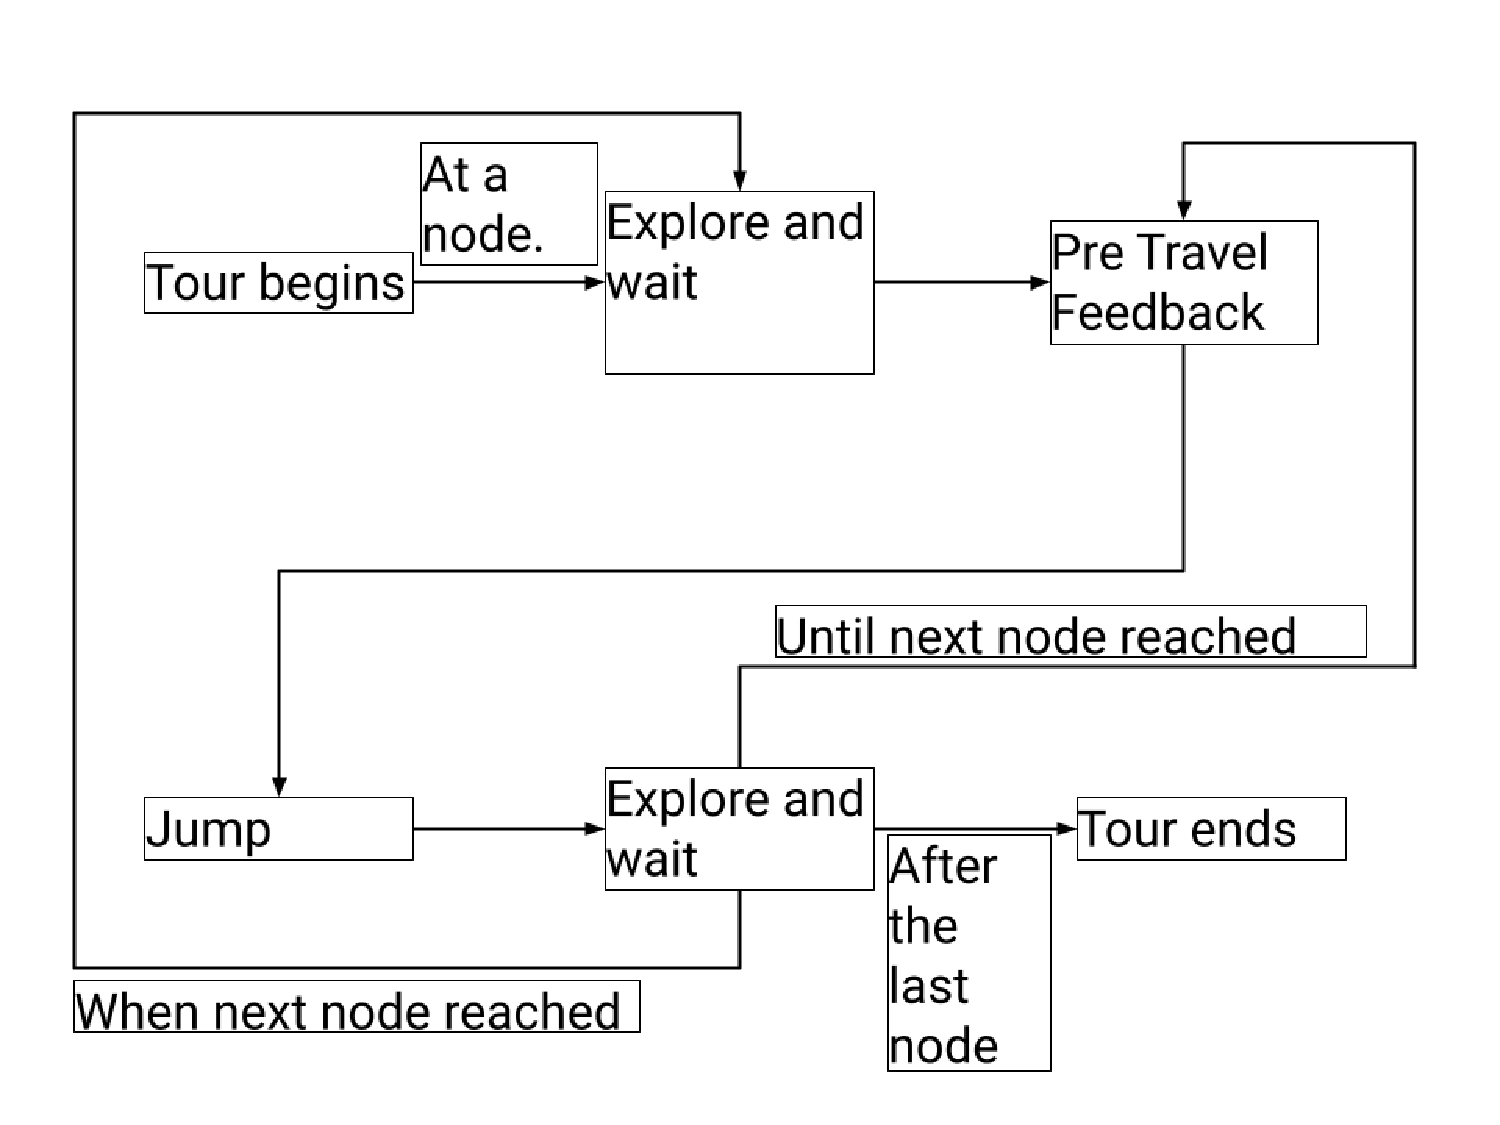
\includegraphics[width=0.5\textwidth]{images/interaction-design-steps.pdf}
	\caption{Steps that would be followed in an exploration of a \acrshort{ve} using the automated guided jumping navigation technique.}
	\label{fig:interaction-design-steps}
\end{figure}

\subsubsection{Travel Feedback}
\label{subsubsection AGJ ID ES: Travel Feedback}
Before a jump takes place, a user needs to know the following information:
\begin{itemize}
	\item The location they will jump to.
	\item Their orientation after the jump.
	\item The time left until the jump takes place.
	\item Whether or not a jump is paused, giving them time to explore.
\end{itemize}

\subsubsection{Pause to Explore}
\label{subsubsection AGJ ID ES: Pause to Explore}
As the jumping is done automatically, it is important to provide the user with some way to control the technique. This can be done by allowing them to somehow pause the jumping either implicitly or explicitly so that they can take the time to explore or look around rather than being worried about automatically moving to the next position. Similarly, users would then also have the ability to implicitly or explicitly to resume once they are ready to continue. Resuming would reset the countdown to a jump so as to avoid sudden jumps after resuming. Looking away from the next node causes the guiding to be paused implicitly and looking back at it can cause the guiding to be resumed as looking around is a natural behavior that someone may use to explore an environment. For explicitly pausing and resuming some form of conscious user input to pause or resume the guiding is required instead.  

\subsubsection{Choice between Nodes}
\label{subsubsection AGJ ID ES: Choice between Nodes}
In addition to users having the option to pause, users should also have some control over the path they take. This can be provided by adding some nodes where a choice is given to the users between multiple possible nodes they can go to. Information and travel feedback about each node is given to the users and then they can select their preferred node from the given options. 

\section{Environment Setup}
\label{section AGJ: Environment Setup}

Once we came up with a suitable interaction design for the technique we had to decide how an environment would need to be set up to use this technique. Figure \ref{fig:interaction-design-layout} shows a basic environment in which our guided jumping technique can be used. As mentioned in subsection \ref{subsection AGJ ID: Exploration Steps}, a user has to travel from one node to the next. As nodes are points of interest and can be far apart from each other, to ensure short jumps there are way points between them. The figure \ref{fig:interaction-design-layout} shows these nodes as and way points as black and yellow spheres respectively. As we see in \ref{subsubsection AGJ ID ES: Choice between Nodes}, sometimes there can be more than one node to choose from as the next node. This is indicated in the figure through numbers and arrows.     
\begin{figure}[]
	\centering
	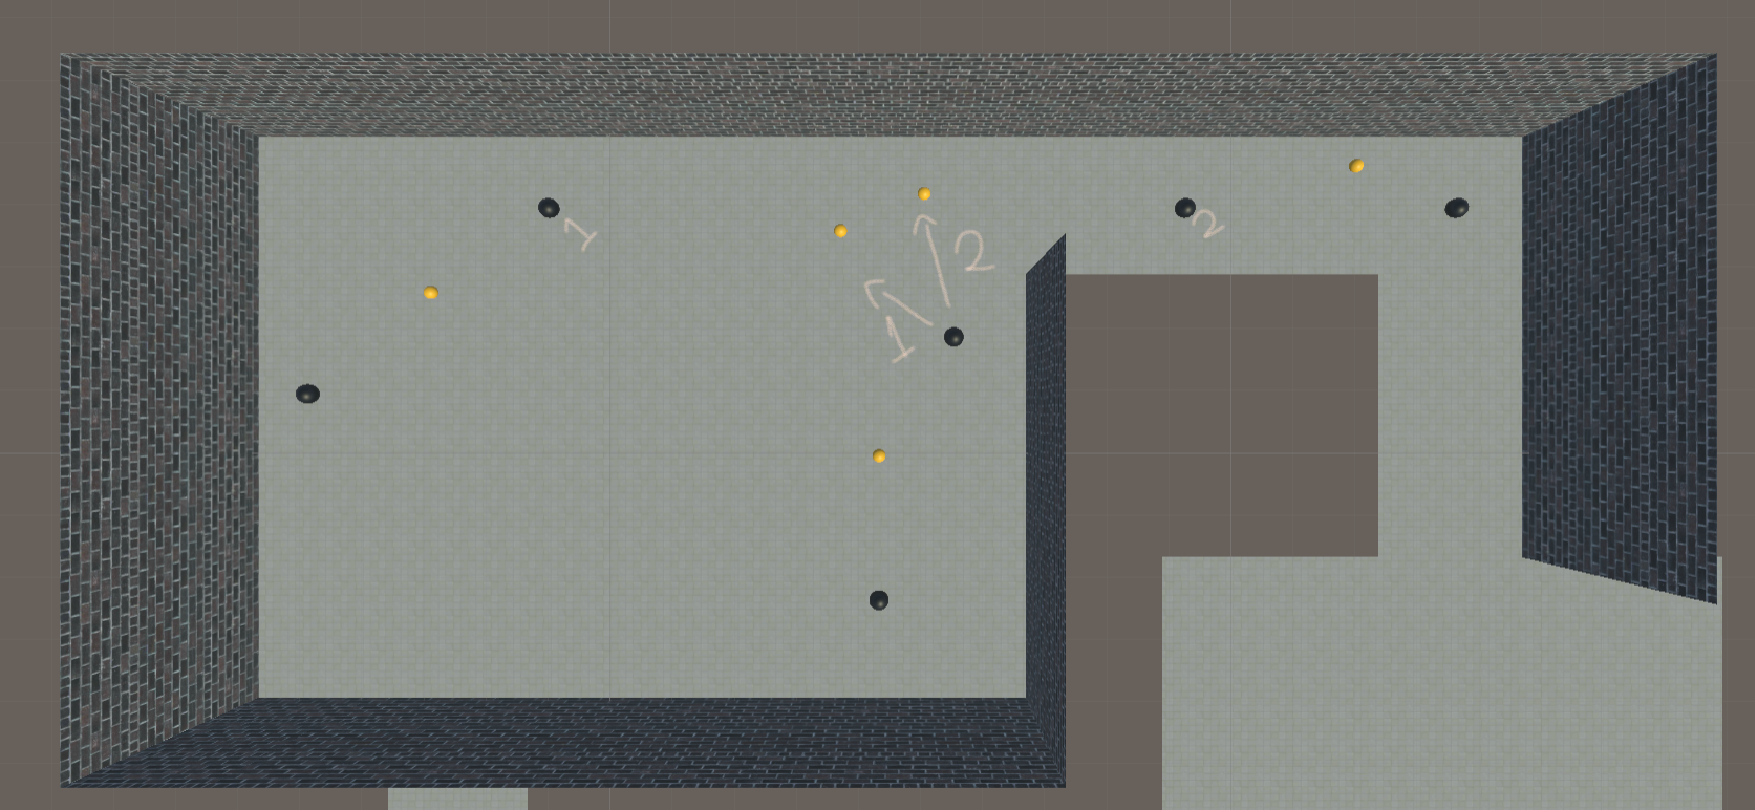
\includegraphics[width=0.5\textwidth]{images/interaction-design-layout.pdf} 
	\caption{This is a potential setup of an environment in which the automated guided jumping navigation would be used. Black spheres = nodes, yellow spheres = way points, arrows and numbers where there is a choice between nodes}
	\label{fig:interaction-design-layout}
\end{figure}

This environment setup with nodes, way points and choices is something that would be a part of the environment design by the creator of an experience or tour. The nodes have to be points of interest so should be placed where there is some exhibit or interesting object for users to look at. Nodes are numbered so that the next node can be linked to a node. Way points should also be setup between the nodes. Lastly, any nodes where there can be a choice between more than one next node is also set up accordingly.
 
\section{Automated Jumping}
\label{section AGJ: Automated Jumping}
Once an environment is setup with nodes and way points automated jumping can be carried out by moving a user from each way point or node to the next while keeping in mind important aspects of teleportation techniques as specified by Weissker et al. These are \textit{'target specification, pre-travel information, transitions and post-travel feedback'}~\cite{Weissker2018} and are what make the jumps comprehensible.

\subsection{Comprehensibility of Jumps}
\label{subsection AGJ AJ: Comprehensibility of Jumps}
The target specification in this case is automatic and has been preassigned as the next node or way point, except for when there is a choice between more than one way point or node as the next target. Pre-travel information is provided as avatars positioned at the target's location and facing the direction that a user would be oriented towards after a jump. In addition, the time left till the jump will take place is also indicated by a line that gets narrower as less time is left. This can be seen in figure \ref{fig:automated-jumping-feedback}. We decided to go with simple instant transitions for the jumps. There is no specific post-travel feedback, however, after a jump users can already see the pre-travel information for the next jump and are therefore aware that they have completed the current jump. 

\begin{figure}[]
	\centering
	(\centering 1) {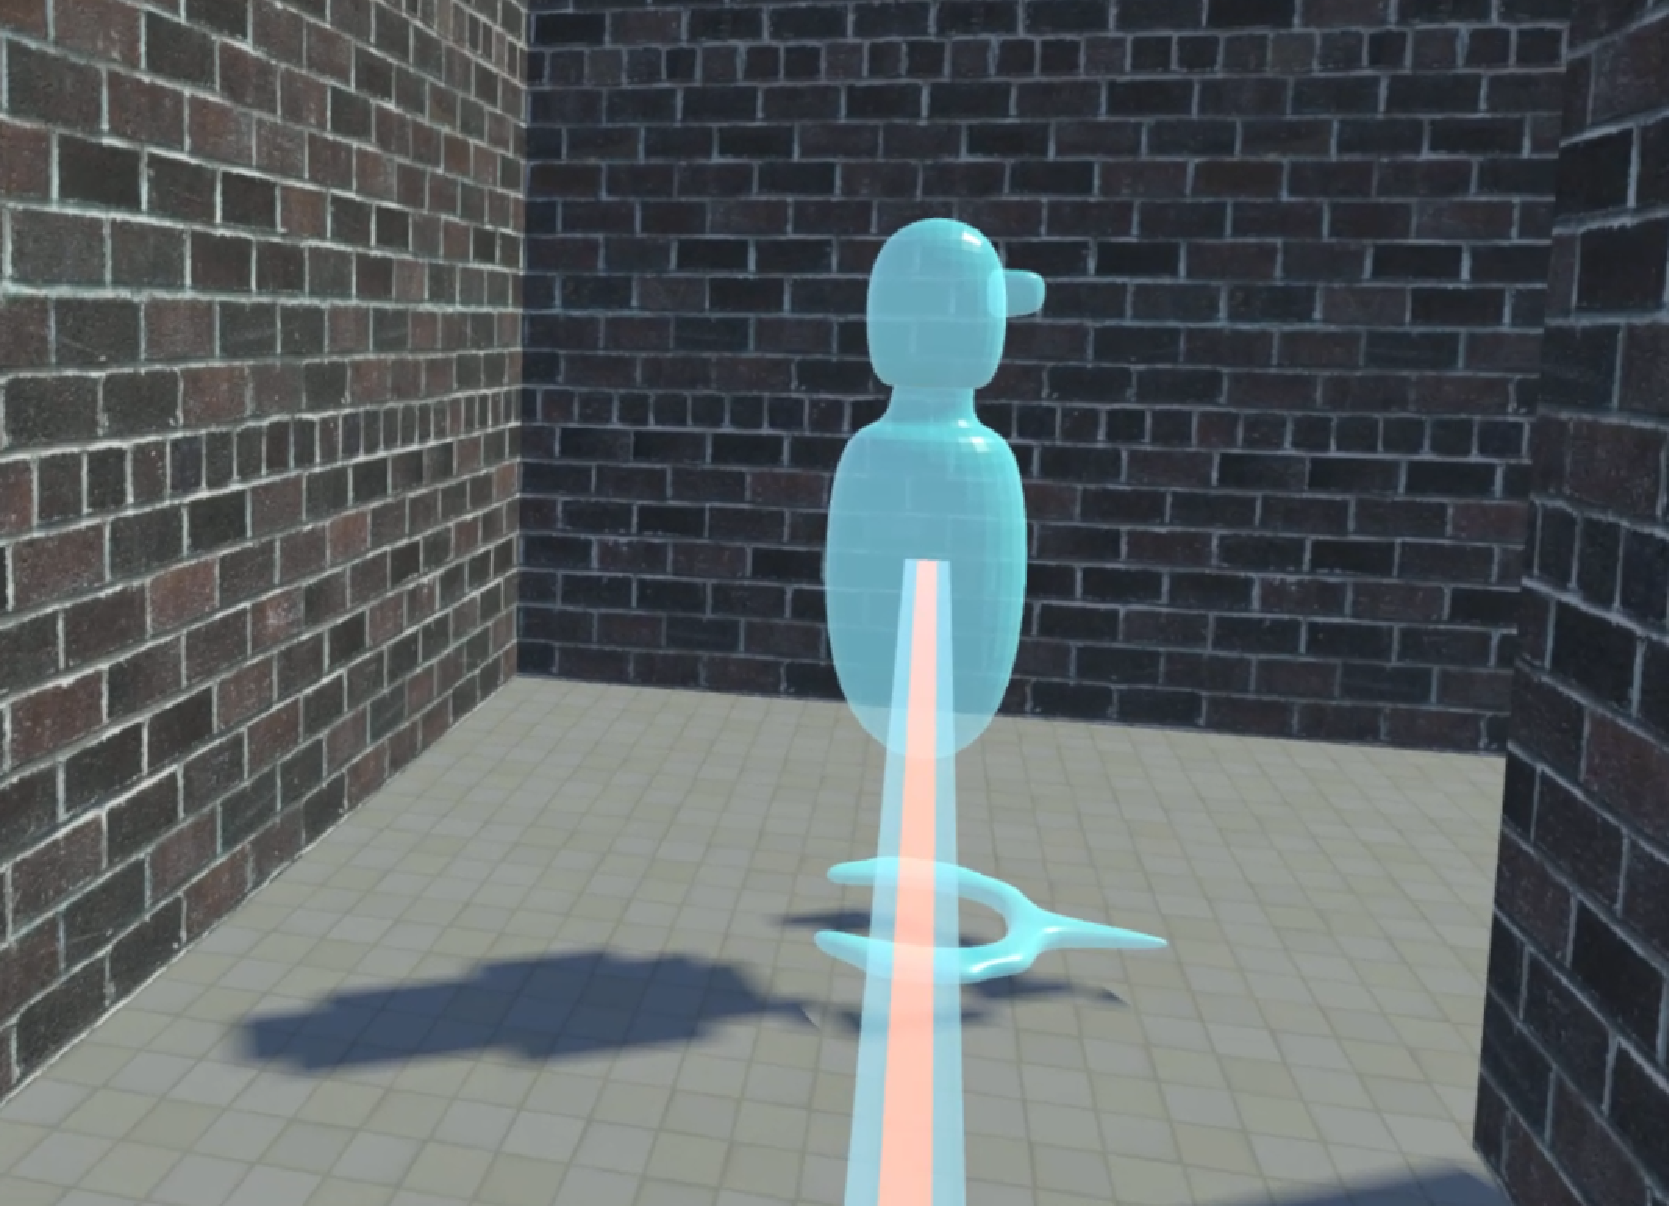
\includegraphics[width=0.25\textwidth]{images/automated-jumping-feedback-1.pdf}}
	(\centering 2) {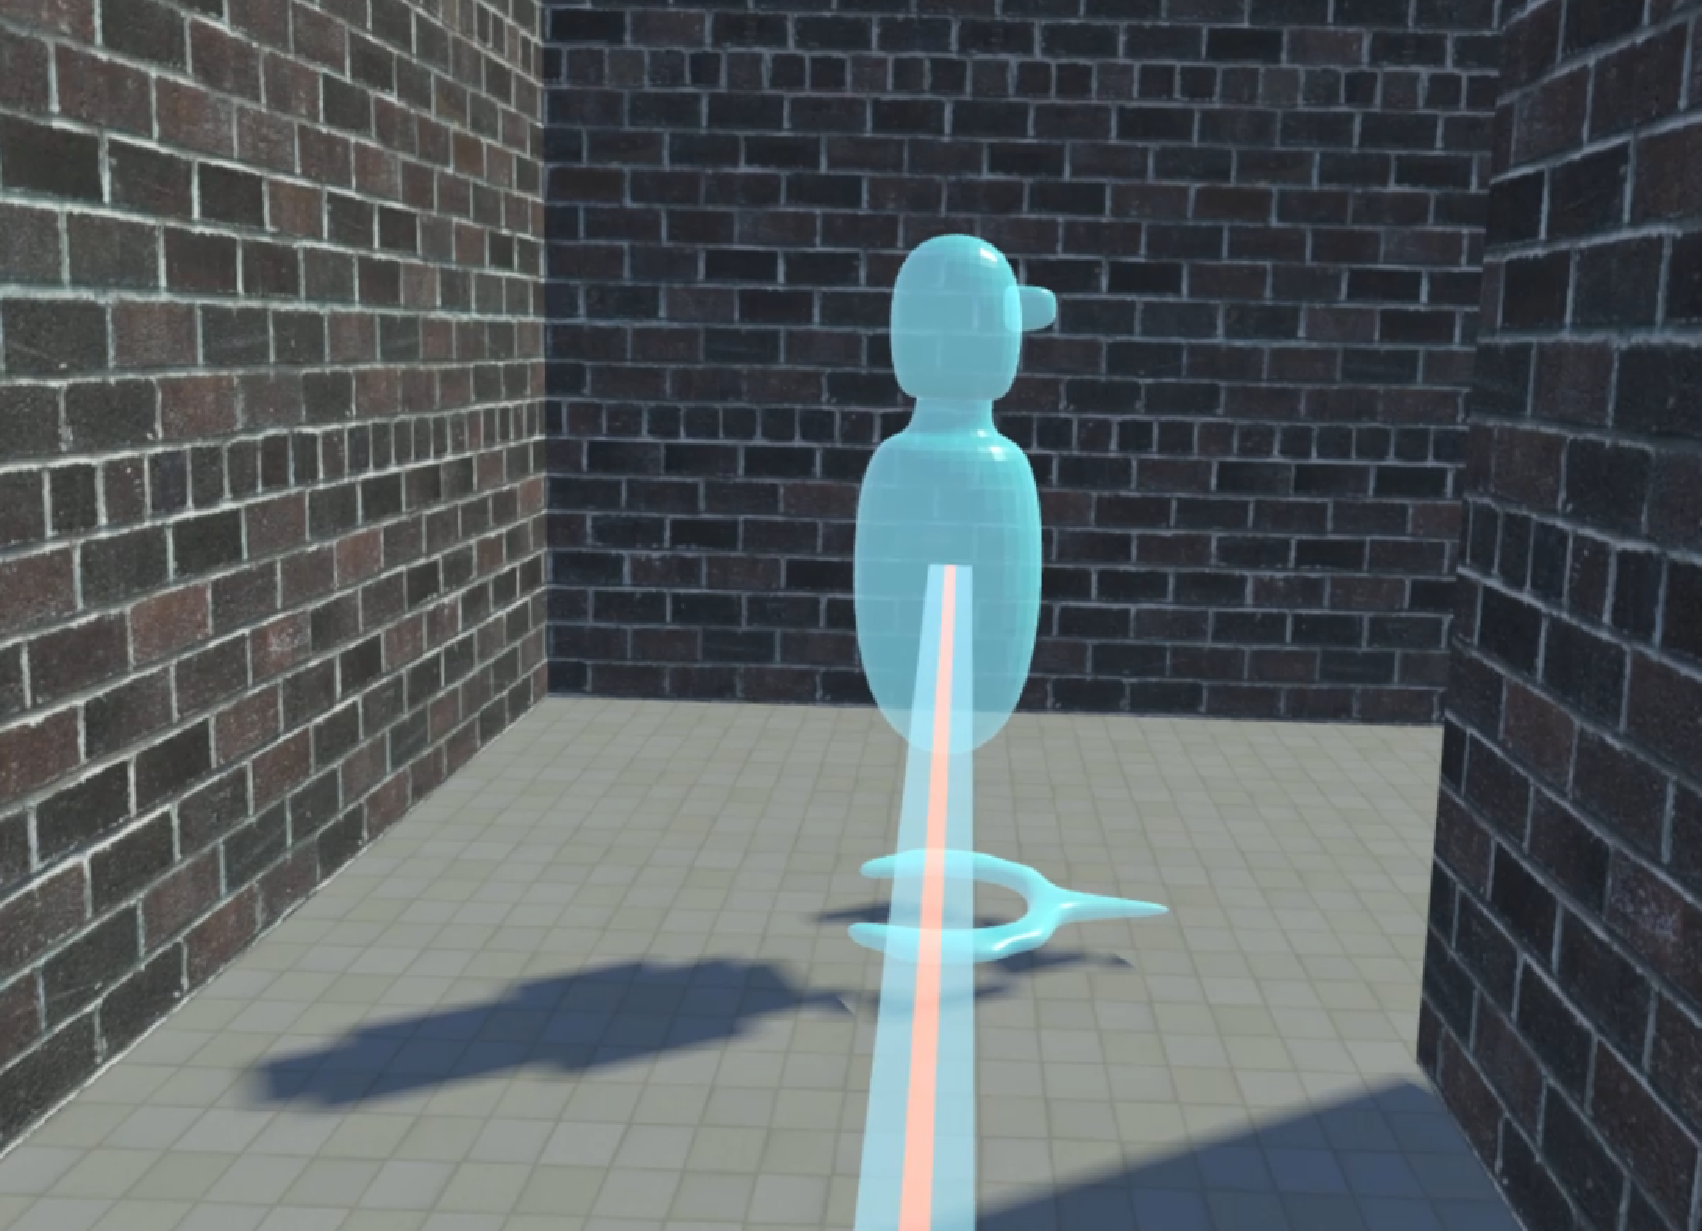
\includegraphics[width=0.25\textwidth]{images/automated-jumping-feedback-2.pdf}} 
	\caption{Avatar at target position facing orientation the user will face after jump. The orange line can be seen to decrease in width between (1) and (2) indicating time left till jump.}
	\label{fig:automated-jumping-feedback}
\end{figure}  

Finally, there has to be feedback  when the user has to make a choice or when they pause the automated jumping. This feedback is provided through \acrfull{ui}. To indicate a choice needs to be made by the user for what path they want to take, there is a combination of arrows and signs pointing to the avatars that indicate the next possible positions to choose from. On selection a sign that says \textit{'Selected!'}is used to show which option has been selected. In addition, the arrow and sign for the option that is not selected disappear. Once feedback has been given for making a choice, the guiding continues with the node or way point represented by the selected avatar as the next node or way point. To indicate that the automatic guiding is paused, a sign that says \textit{'Paused'} becomes visible. Figure \ref{fig:automated-jumping-feedback-ui} shows these different \acrshort{ui}s for feedback on pausing or making a choice. 

\begin{figure}[]
	\centering
	(\centering 1) {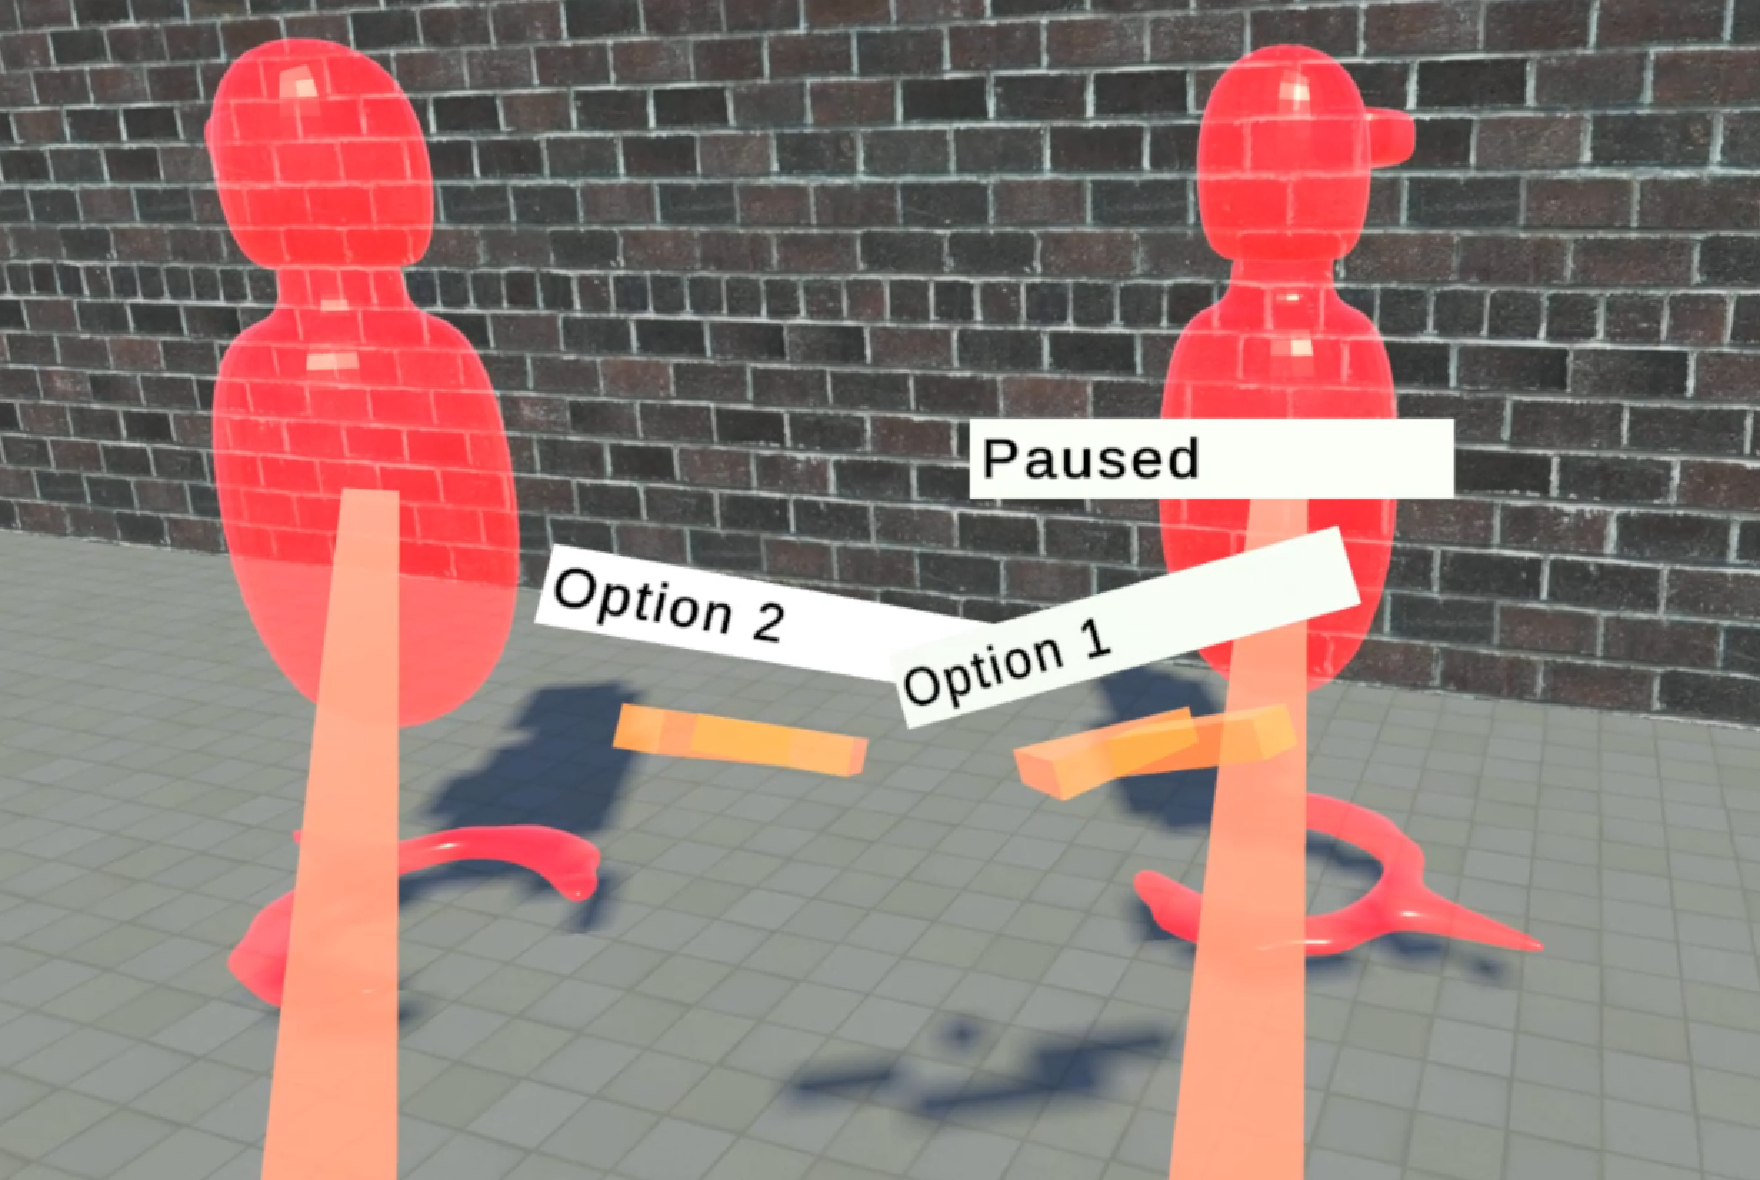
\includegraphics[width=0.25\textwidth]{images/choose.pdf}}
	(\centering 2) {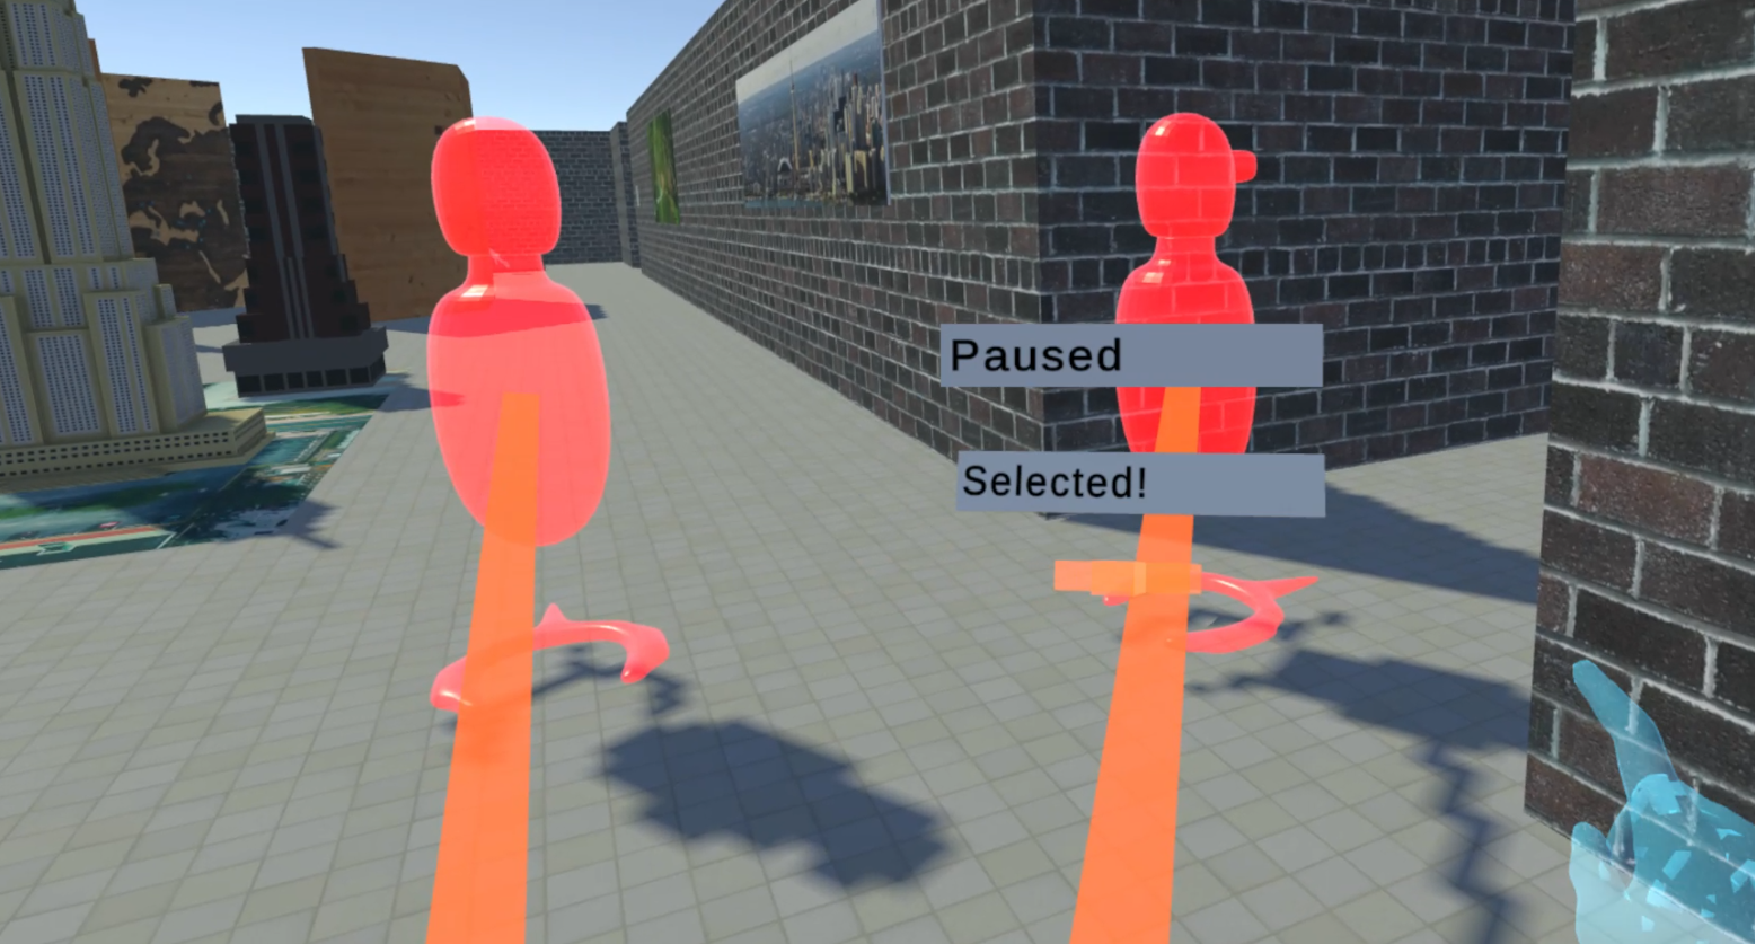
\includegraphics[width=0.25\textwidth]{images/choice-made.pdf}}
	(\centering 3) {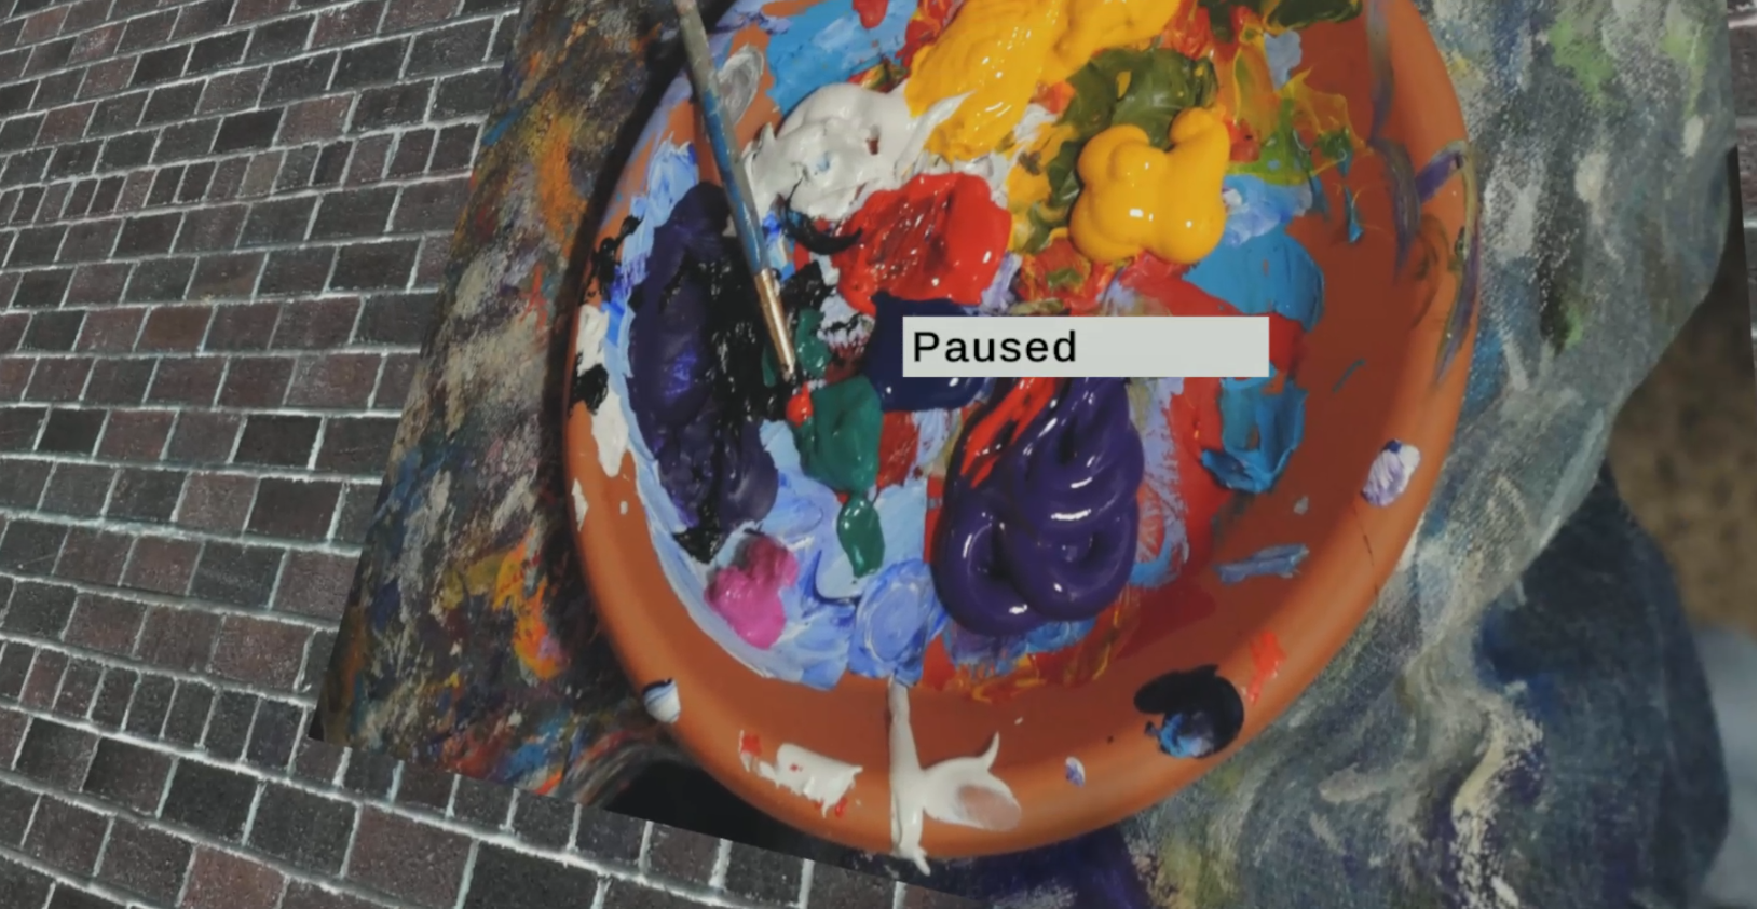
\includegraphics[width=0.25\textwidth]{images/paused.pdf}} 
	\caption{Feedback when making a choice or pausing: (1) Arrows and signs pointing to the different avatars indicating a choice. (2) The selected avatar is indicated by a sign while the arrow and sign for the avatar not selected disappear. (3) A sign showing that automated jumping has been paused.}
	\label{fig:automated-jumping-feedback-ui}
\end{figure} 

\subsection{Gesture Control}
\label{subsection AGJ AJ: Gesture Control}
Since we wanted to reduce the learning difficulty for users and also the hardware that would be required to use the technique, we decided on allowing users to use hand gestures with a \acrshort{hmd} that allows for gesture tracking. Users can pause and resume the automated guiding explicitly through hand gestures. They can also use a pointing hand gesture to choose the next node or way point when there is a choice between more than one. These hand gestures should be natural and represent how a person may do a similar action in a non-virtual environment. Figure \ref{fig:automated-jumping-gestures} shows the hand gestures being used in our \acrshort{ve} using an Oculus Quest.
\begin{figure}[]
	\centering
	(\centering 1) {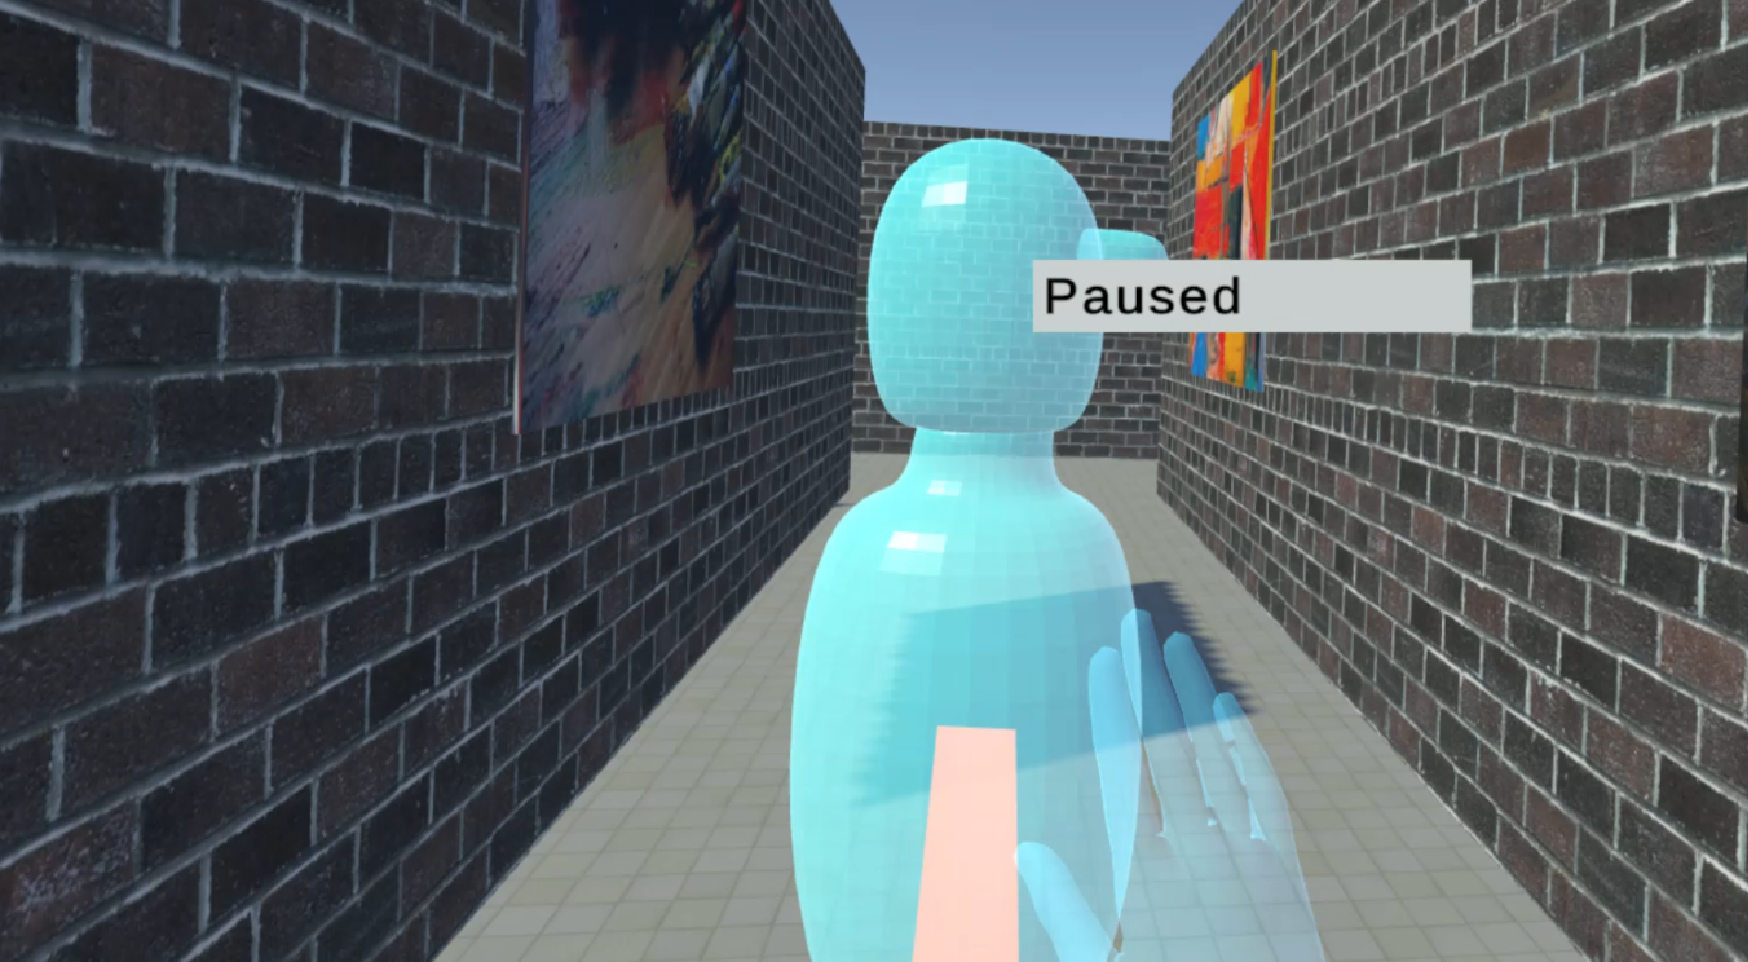
\includegraphics[width=0.25\textwidth]{images/paused-gesture.pdf}}
	(\centering 2) {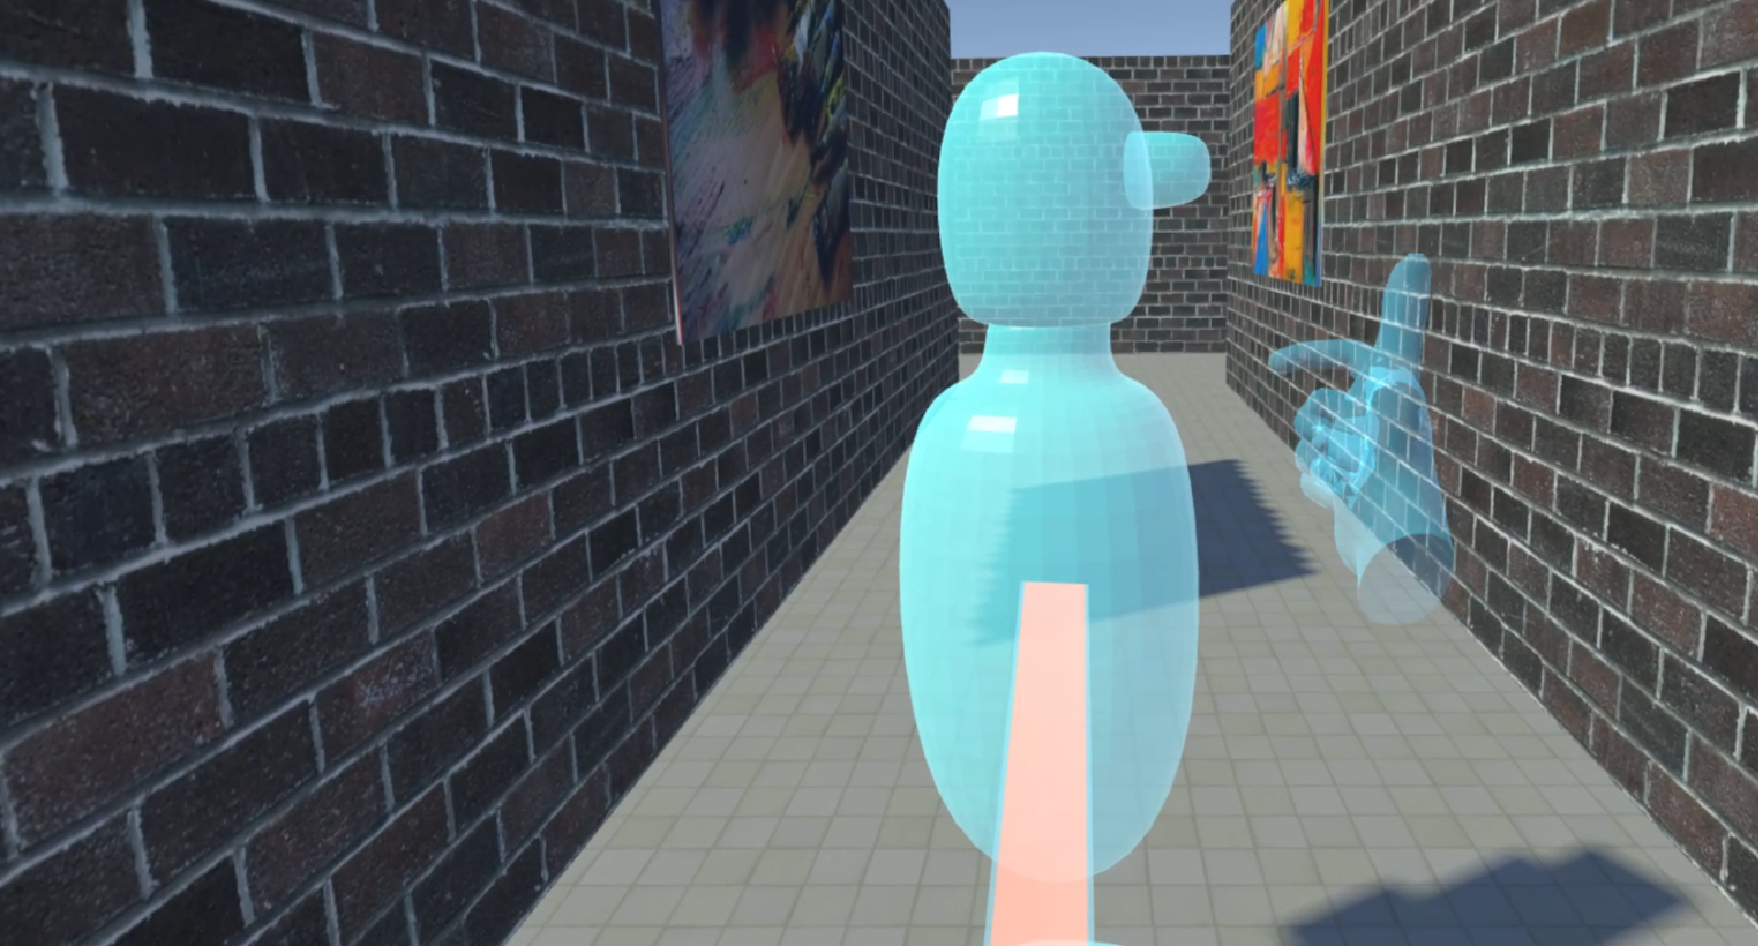
\includegraphics[width=0.25\textwidth]{images/resume-gesture.pdf}}
	(\centering 3) {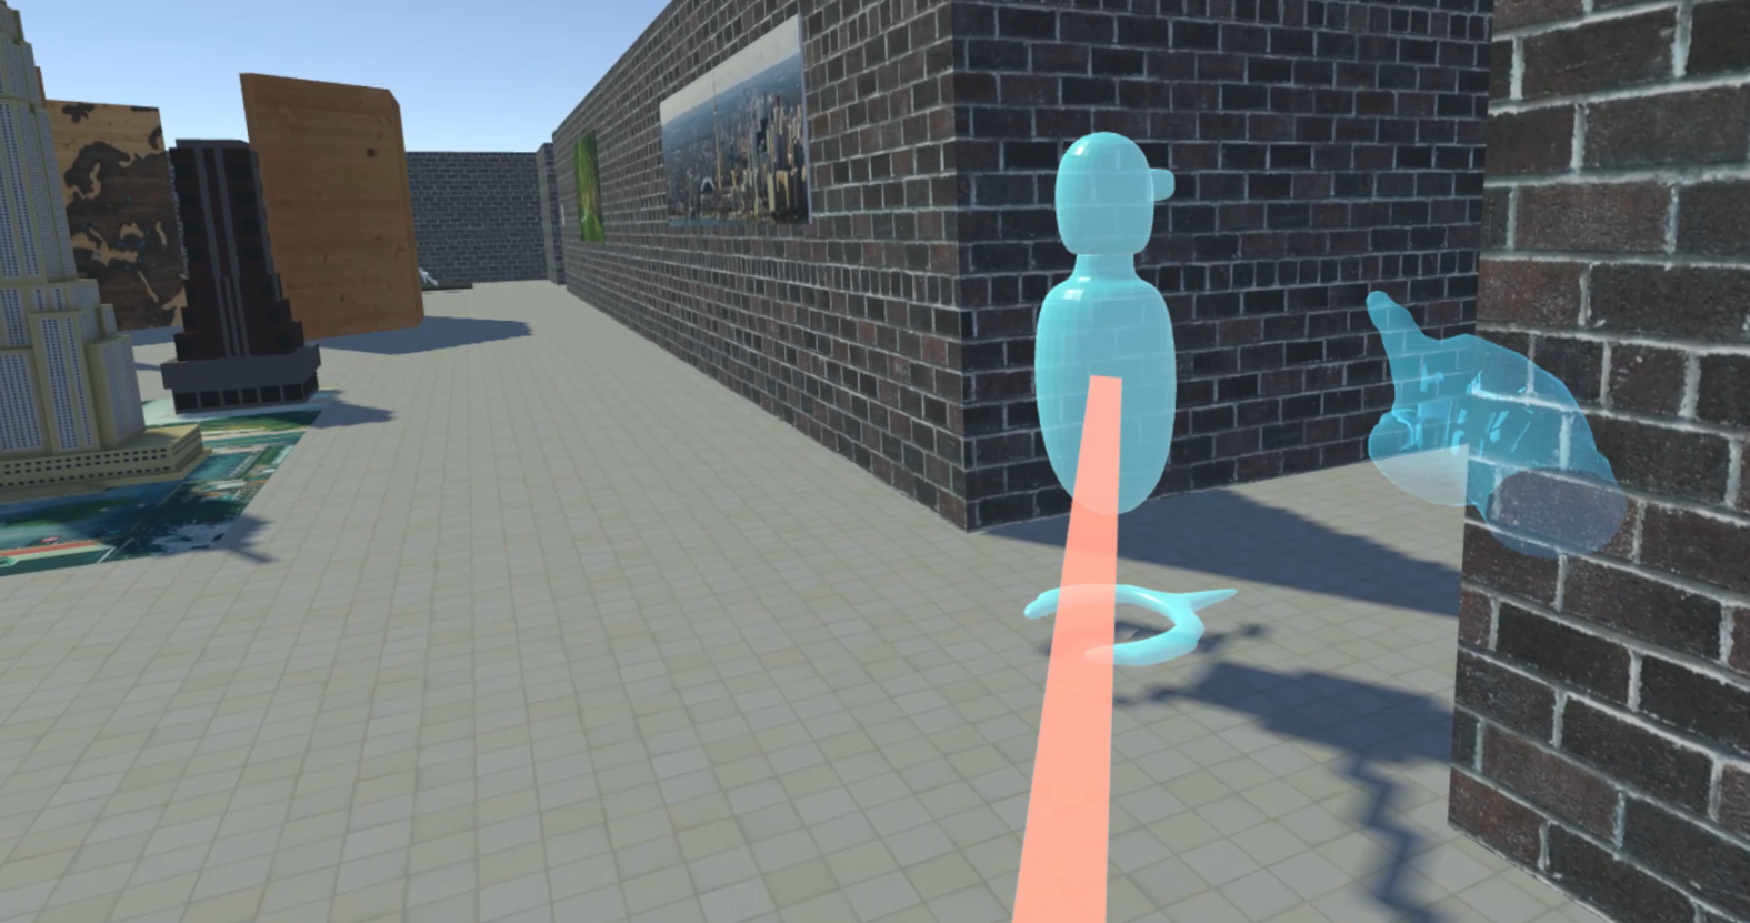
\includegraphics[width=0.25\textwidth]{images/choice-gesture.pdf}} 
	\caption{Gesture control to (1) pause, (2) resume and (3) make a choice.}
	\label{fig:automated-jumping-gestures}
\end{figure} 

%%%%%%%
% Design of the User Study
%%%%%%%

\chapter{Design and Procedure of the User Study}
\pagenumbering{arabic}
\label{Chapter:Design and Procedure of the User Study}
\section{Hypotheses}
\label{section DPUS: Hypotheses}
In \cref{Chapter:Automated Guided Jumping} we looked at a technique for automated guided navigation using the jumping metaphor and we also saw how the jumps in this technique could be made comprehensible so that the user would know when and where they will jump. The motivations and scenarios that might require such a technique were discussed in \cref{Chapter:Guided Jumping Motivation}. Keeping in mind the motivation to have a virtual museum that novice \acrshort{vr} users are able to explore we came up with the research questions \cref{rq:rq1}, \cref{rq:rq2} and \cref{rq:rq3} that are mentioned in \cref{section GJM: Conclusion}.

To study the developed technique with regards to these research questions we decided to design a study that would compare our developed technique for automated guided jumping with a user controlled (free) jumping technique having visual guidance. With this study we hoped to prove the following hypotheses:

\begin{hypothesis}
	\label{hyp:hyp1}
	Participants do not get more simulator sickness while using the automated guided jumping compared to free jumping with visual guidance.
\end{hypothesis}
\begin{hypothesis}
	\label{hyp:hyp2}
	Visual previews before automated jumps will have similar comprehensibility of the jumps compared to free jumping with visual guidance.
\end{hypothesis}
\begin{hypothesis}
	\label{hyp:hyp3}
	Automated guided jumping will reduce task load compared to free jumping with visual guidance.
\end{hypothesis}
\begin{hypothesis}
	\label{hyp:hyp4}
	Users will be able to recall their path when using automated guided jumping as well as when free jumping with visual guidance.
\end{hypothesis}

Hypothesis \cref{hyp:hyp1} is important because we want to justify the need for automate the guided jumping without compromising on the reason for using jumping as the navigation metaphor, that is reduced motion sickness. To also justify that spatial awareness is similar in our technique versus free jumping the study must prove \cref{hyp:hyp2} and \cref{hyp:hyp4}. \cref{hyp:hyp2}  also needs to be proved to show that the technique is easy to understand and users will not get confused when using it compared to free jumping. In order to prove the benefit of automated guided jumping over free jumping with visual guidance the study must show that \cref{hyp:hyp3} is true.  

\section{Study Task and Limitations}
\label{section DPUS: Study Task and Limitations}
As the study will be comparing automated jumping with free jumping using visual guiding, it was important to plan a controlled study design such that there would be no other influencing variables besides the automation. Therefore, when developing the free jumping technique that would be used for comparison we had to make sure that the only difference between it and our automated jumping technique would be that the user would make the jumps themselves instead of being automatically moved. There are still nodes and way-points in the scene that are used to show visual guidance with an avatar being visible at the next node and a path drawn through way-points as in \cref{fig:study-free-jumping}. The figure also shows the teleportation indicator with a curve pointing to it that users can use to select the position and orientation they want to be at after the jump.

\begin{figure}[]
	(\centering 1)
	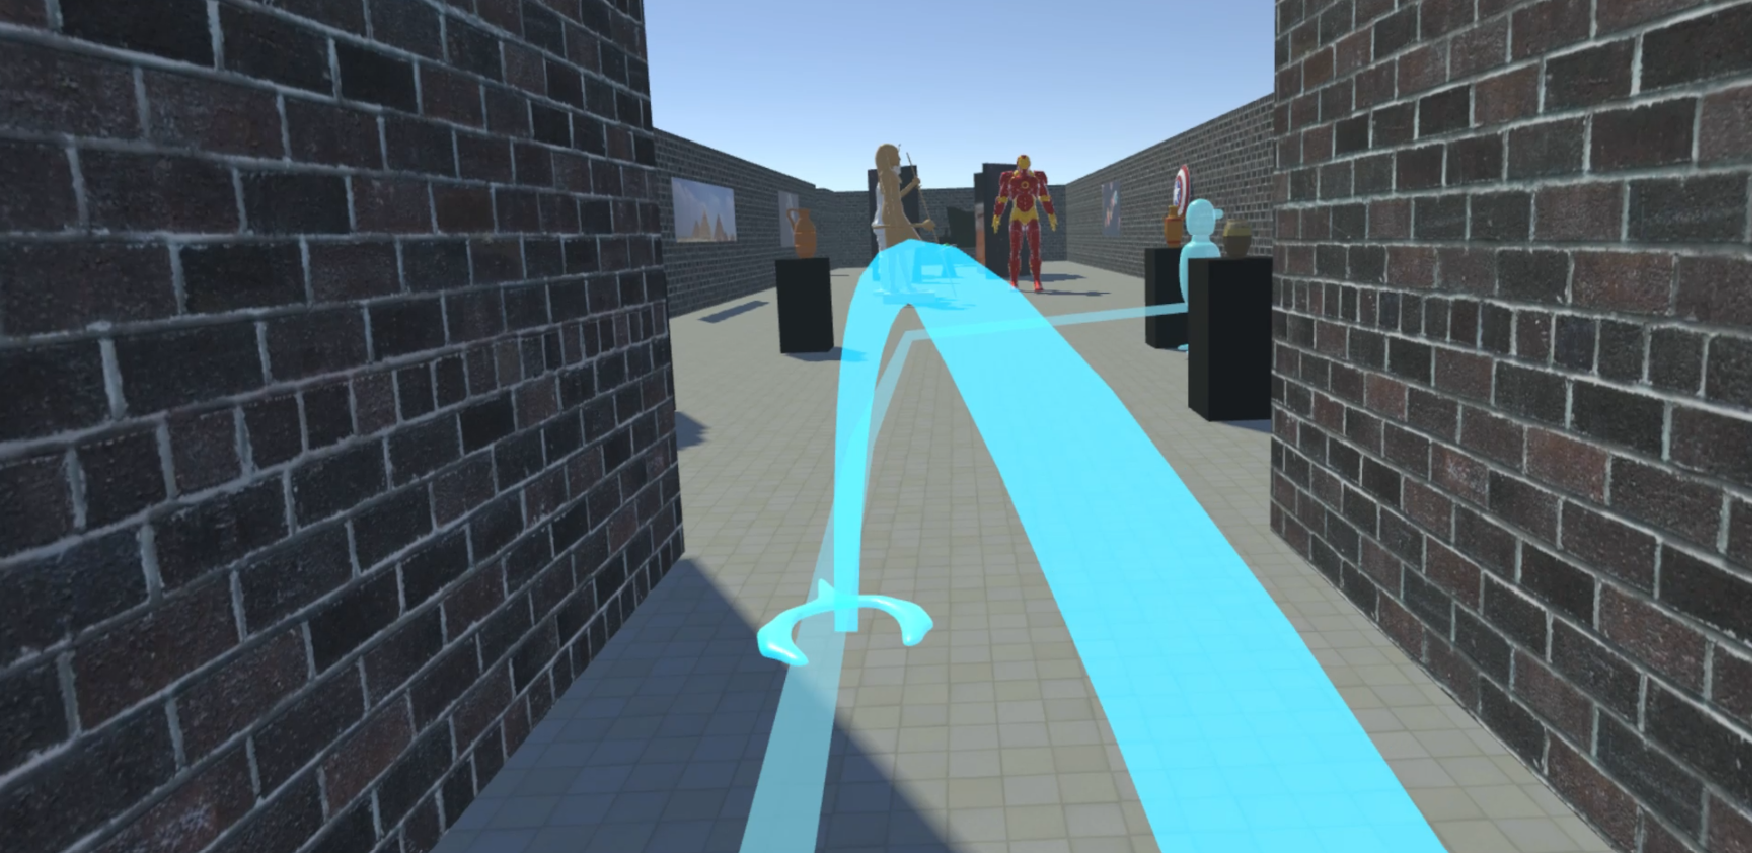
\includegraphics[width=0.25\textwidth]{images/free-jumping.pdf}
	(\centering 2)
	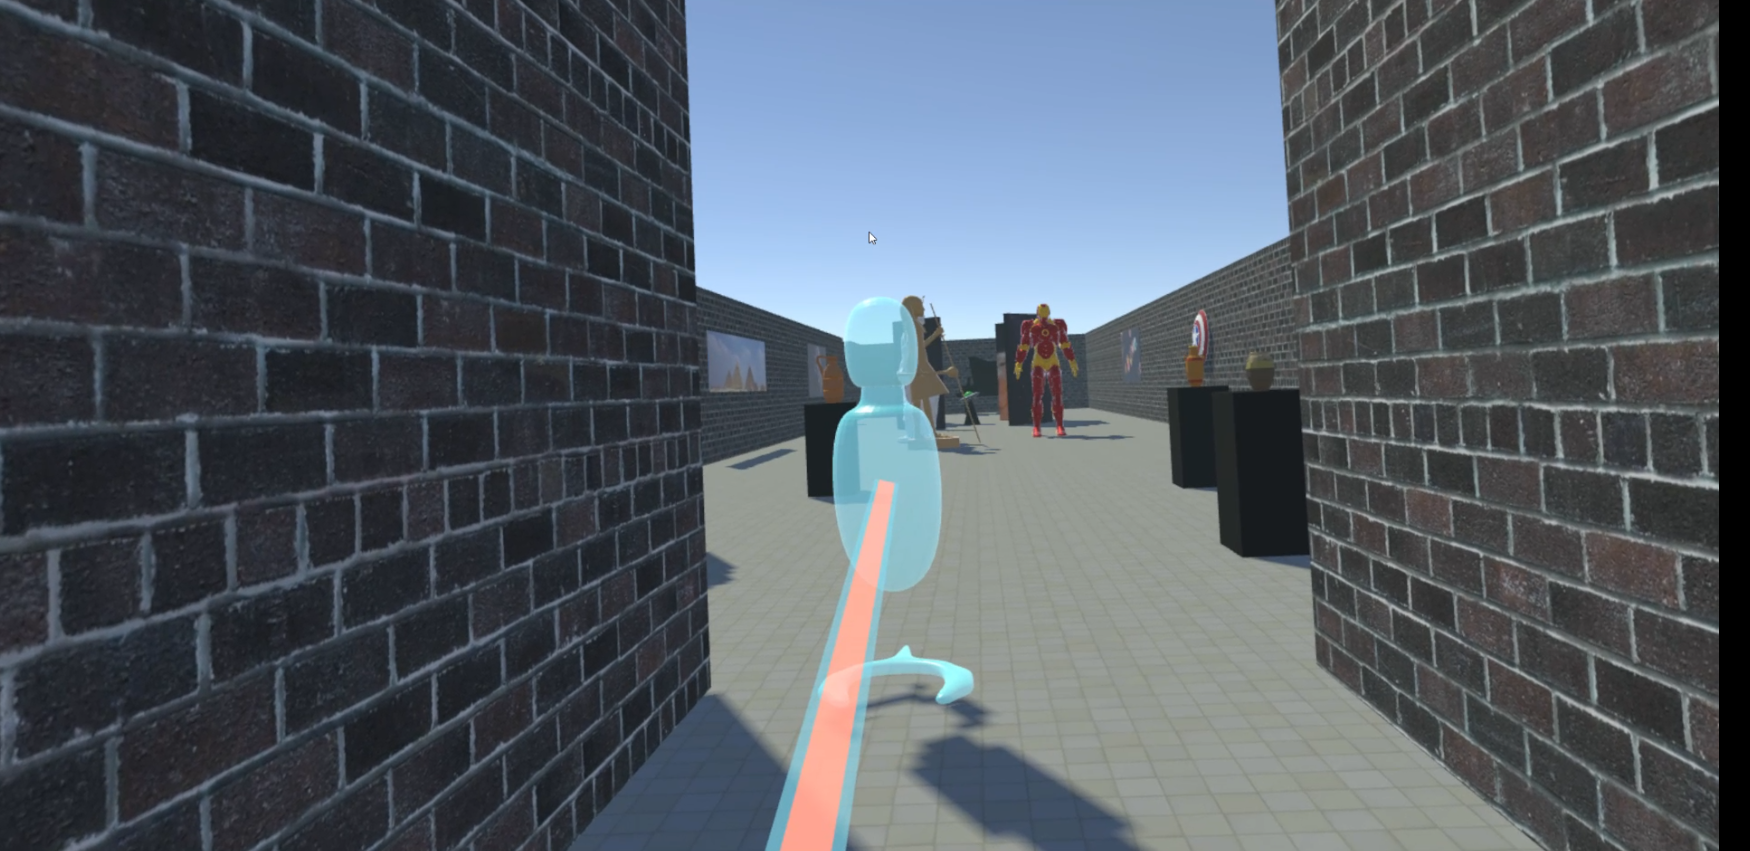
\includegraphics[width=0.25\textwidth]{images/automated-jumping.pdf}
	\caption{Free jumping with visual guidance.}
	\label{fig:study-free-jumping}
\end{figure}

As discussed in \cref{section GJM: Virtual Tours} one of the use cases for guiding techniques is virtual tours and we developed our technique for such a scenario as mentioned in \cref{subsection AGJ ID: Scenario}. Therefore, the study design also kept in mind a virtual tour situation and considered the potential problem situations that may occur and the possible tasks that may be expected when touring through a virtual space. For this study the task was narrowed to touring a virtual museum with exhibits and trying to remember the path taken as well as the objects seen. This is a useful task when going through a museum and gives answers about whether the techniques used are facilitating acquisition of relevant knowledge of the scene as we hoped to do so through our technique and can be seen in \cref{rq:rq1}.

This task situation for this study will not cover all possible situations that may arise when taking a virtual tour such as:
\begin{itemize}
	\item Exhibits that are very close or far from each other.
	\item More than 2 possible paths to choose from at some nodes.
\end{itemize} 

\section{Variables and Conditions}
\label{section DPUS: Variables and Conditions}
Keeping in mind the task of touring a museum and remembering the path and objects, there are certain variables that need to be varied between the two techniques and others that need to be measured. 

\subsection{Independent Variables}
\label{subsection DPUS VC: Independent Variables}
As we saw in \cref{section DPUS: Study Task and Limitations}, automation is the only variable that should be different between the two techniques that are being compared. This means that one technique will have automated jumping and the other will not but the visual guidance and ability to have a choice must remain the same. In addition it is important to keep the number of nodes and way-points the same. It is also necessary to keep the environment and objects of similar complexity. 

\subsection{Dependent Variables}
\label{subsection DPUS VC: Dependent Variables}
The variables that would depend on whether the technique is automated or not are related to the hypothesis that we introduced in \cref{section DPUS: Hypotheses}. The amount of simulator sickness needs to be measured somehow to answer \cref{hyp:hyp1}. A higher amount of simulator sickness is undesirable while lower amounts are better. \cref{hyp:hyp2} can only be answered by finding some way to determine comprehensibility of jumps. The more comprehensible users find a jump the better. The variable needed to answer \cref{hyp:hyp3} is the task load that users feel they had. A lower task load means that users felt they had to make less effort to complete their task and is, therefore, better. Finally, we also need to measure path recall so that we can prove \cref{hyp:hyp4}. The more a user is able to recall their path the better. We will look into details on how these variables are extracted during the study in \cref{section DPUS: Study Procedure}.

\subsection{Study Conditions}
\label{subsection DPUS VC: Study Conditions}
Since we have two techniques to be compared we decided to go with a within user design with 2 study conditions, one using the automated guiding and the other using free jumping with guidance. To avoid participants recall of the environment after the first condition effecting their recall of the environment for the second condition, it is necessary to have two different but comparable scenes. In addition, to avoid the environment or the study order impacting the results the techniques we decided to alternate the order of the conditions while keeping the environment order the same each time.  
 
\section{Study Procedure}
\label{section DPUS: Study Procedure}
In the previous section we defined variables and conditions for the study. Based on these we planned the study procedure which we will now outline in this section starting with the study setup followed by the study plan.

\subsection{Study Setup}
\label{subsection DPUS SP: Study Setup}
The study setup can be divided into three parts which we will discuss in this section. The hardware setup within a physical space, the virtual environment setup and the user feedback.

\subsubsection{Hardware}
\label{subsubsection DPUS SP SS: Hardware}
As we implemented the technique using hand tracking for the Oculus Quest 2, the study was conducted using this \acrshort{hmd}. The Quest 2 has Oculus Insight technology, which tracks changes in the users' position and orientation without need for external tracking. The play space was set to stationary so that users could remain seated while doing the task as there was no need for physical movement. However, to ensure participants could physically rotate, a revolving chair was setup for them to sit on rather than a stationary one. The participants were also equipped with the Oculus Quest 2 controllers but they only needed to make use of the right controller for the free jumping technique and did not need to use a controller for the automated jumping. The environment was displayed per eye at a resolution of 1832×1920 pixels and with a refresh rate of approximately 72 Hz. The headset was connected with a USB cable through Oculus Link, to a computer running the virtual environment on Unity. An additional laptop computer was also setup so that participants could answer question on it in between the tasks and at the end of the study. There was also some space on the desks with a paper for a drawing task for the path recall, which will be explained more in \cref{subsection DPUS SP: Study Plan} and is linked in the appendix. Finally, the experimenter controlled study conditions via the keyboard connected to the workstation running the environment on Unity. \cref{fig:study-setup} shows a drawing of the physical study environment and setup.

\begin{figure}[]
	\centering 
	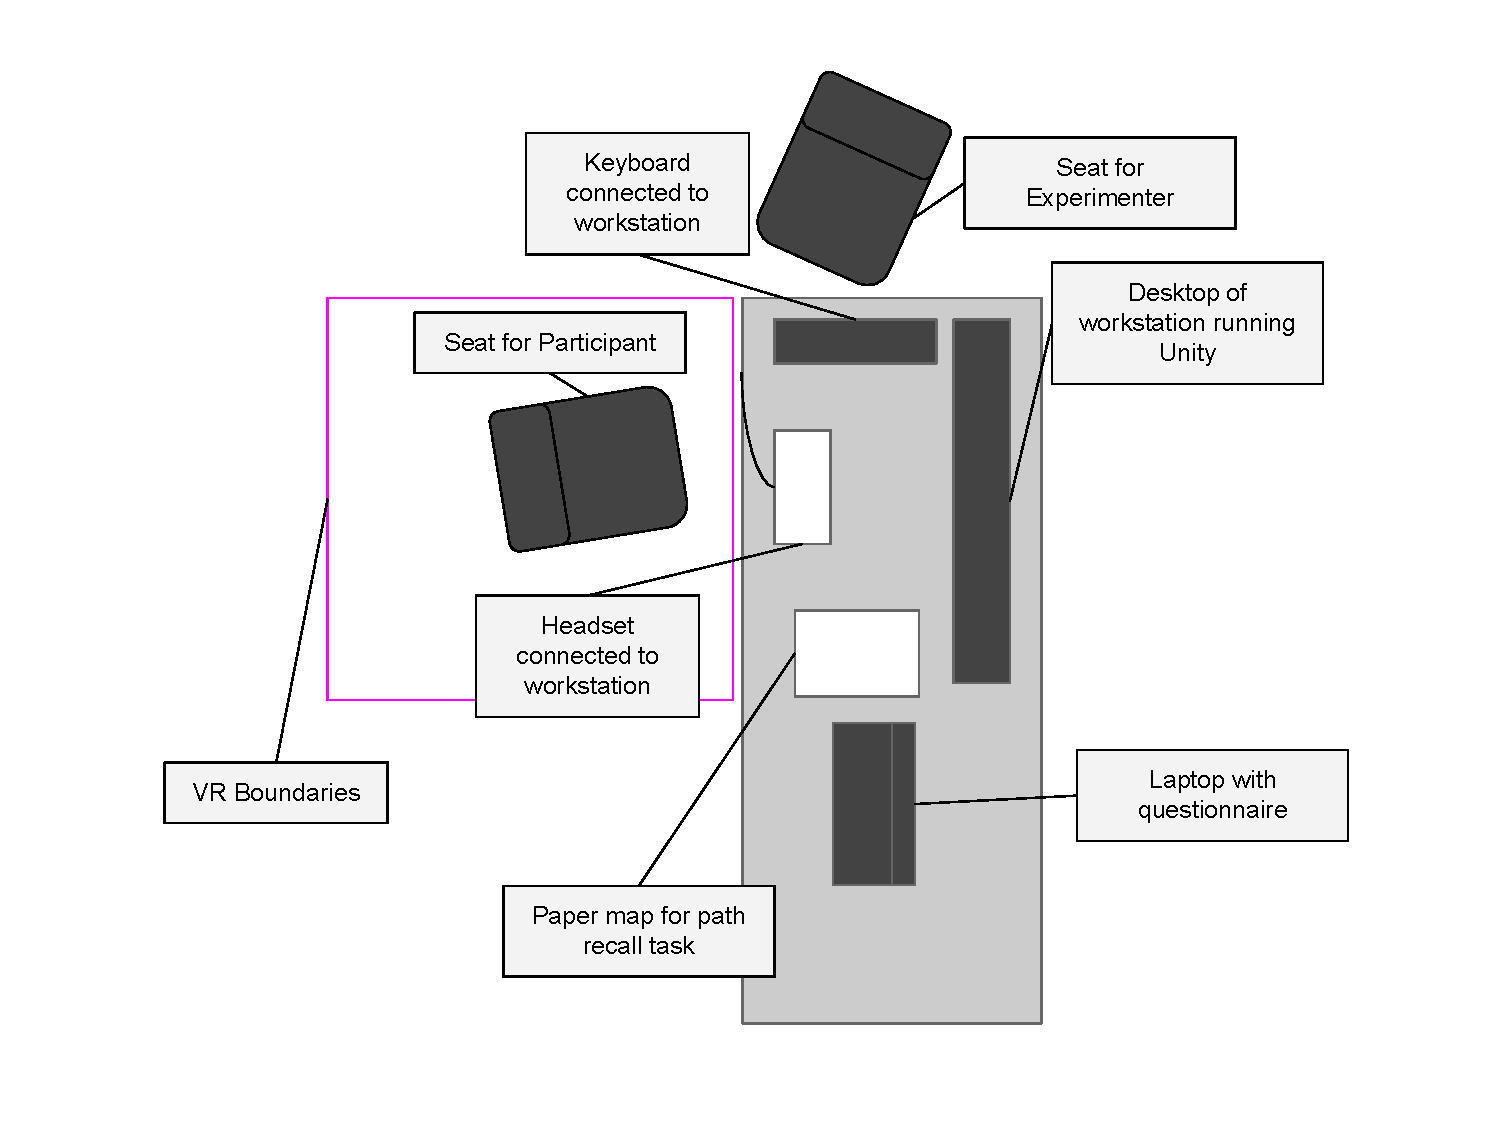
\includegraphics[width=0.8\textwidth]{images/study-setup.pdf}
	\caption{A drawing of the study setup in the Laboratory Space. The experimenter and participant were on the same workspace as the experimenter only needed to use the keyboard.}
	\label{fig:study-setup}
\end{figure}
 
\subsubsection{Virtual Environment}
\label{subsubsection DPUS SP SS: Virtual Environment} 
More than one virtual environment was used for the study. These could be divided into rooms between which the user would switch once each part of the study was conducted. There was one tutorial room in which tutorials for both techniques would take place. There were then two other rooms which were the actual environment for the study tasks. These rooms were a simple museum setup with three rooms connected by one T-shaped corridor and two simple corridors. The rooms had a number of exhibits with a total of 11. There were also 15 paintings distributed along the walls of the rooms and corridors. There are a total of 12 nodes with 29 way-points unevenly distributed between them. There is a choice between 2 nodes at the $5^{th}$ node meaning that participants only end up going through 8 nodes with 19 unevenly distribute way-points in one tour. Top down views of these three rooms can be seen in \cref{fig:study-environment}. Room B is a mirror of Room A but has different exhibits and paintings. The node and way point placement order is also a little different but the number of nodes and distribution of way-points among nodes is the same. The node at which the choice is to be made between 2 nodes is also the same. 

\begin{figure}[]
	(\centering 1)
	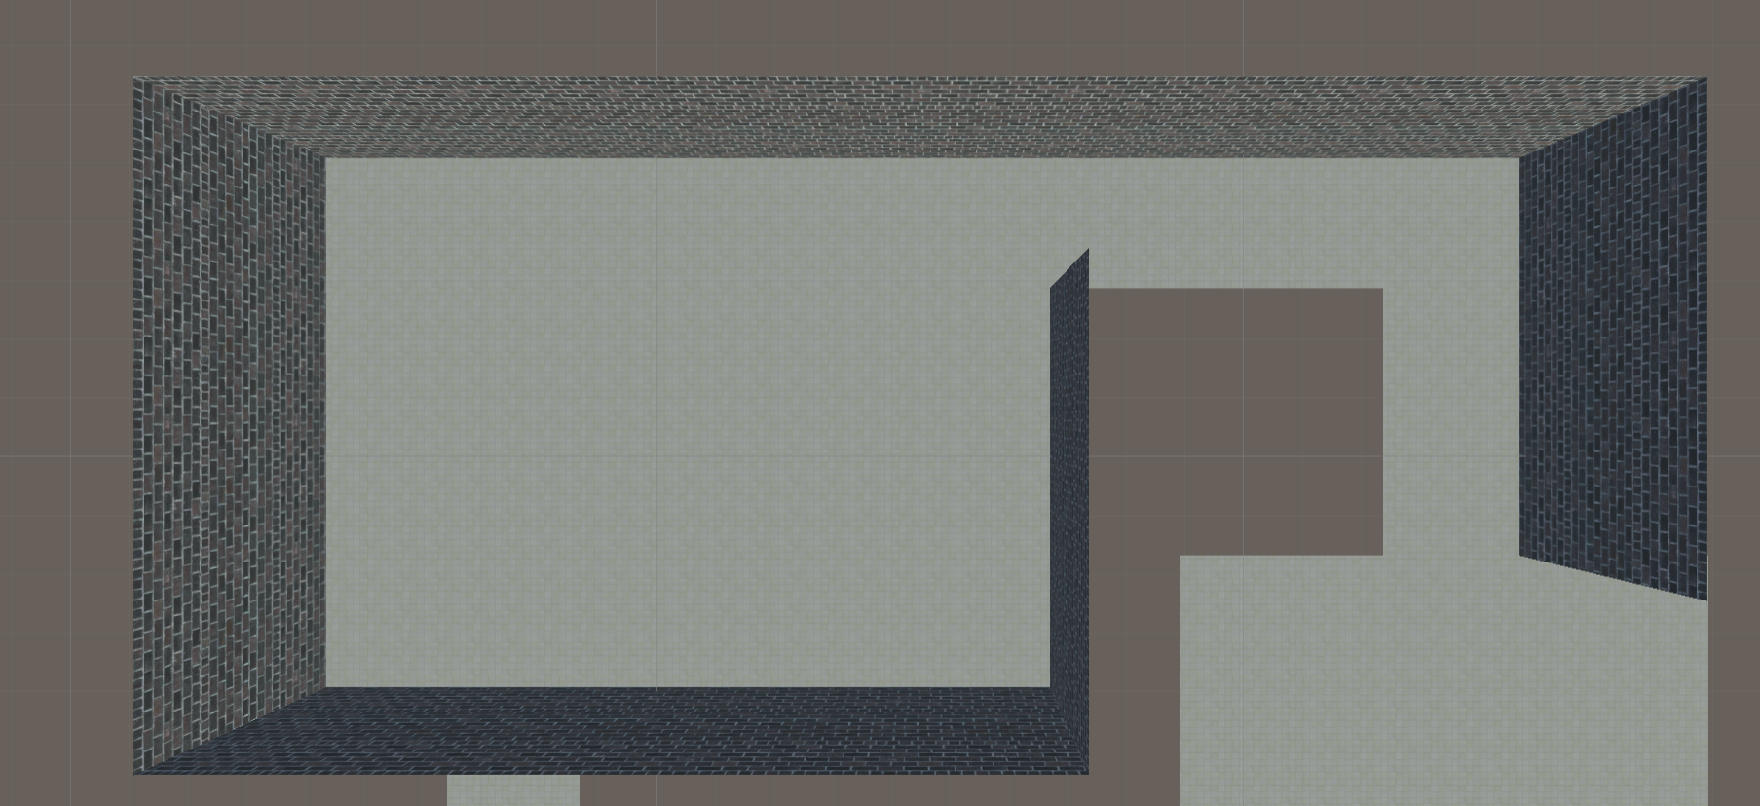
\includegraphics[width=0.25\textwidth]{images/tutorial-room.pdf}
	(\centering 2)
	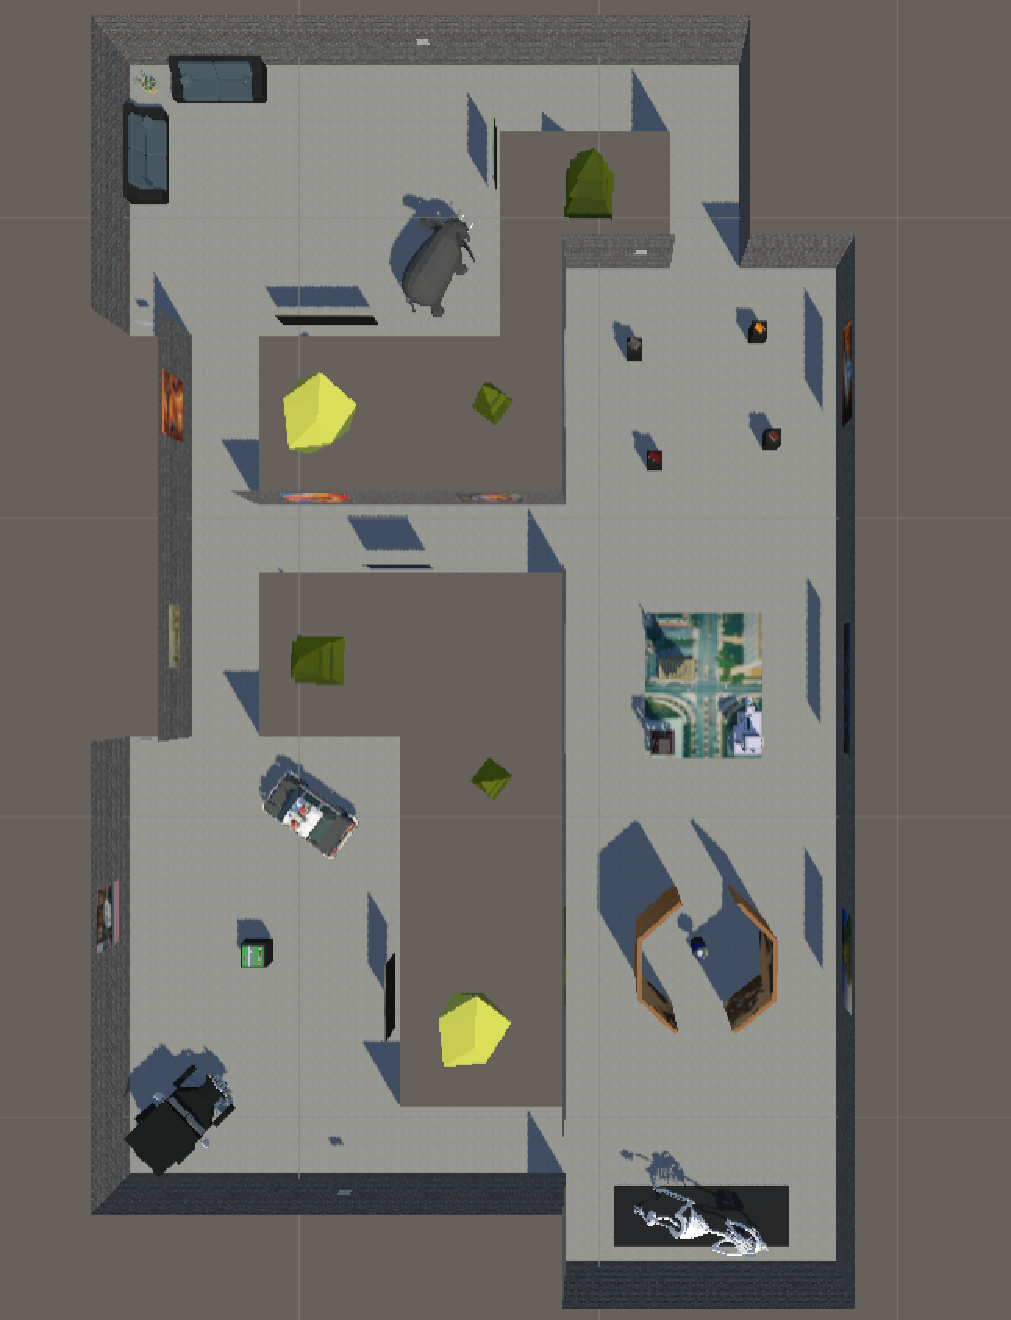
\includegraphics[width=0.25\textwidth]{images/museum-1-objects.pdf}
	(\centering 3)
	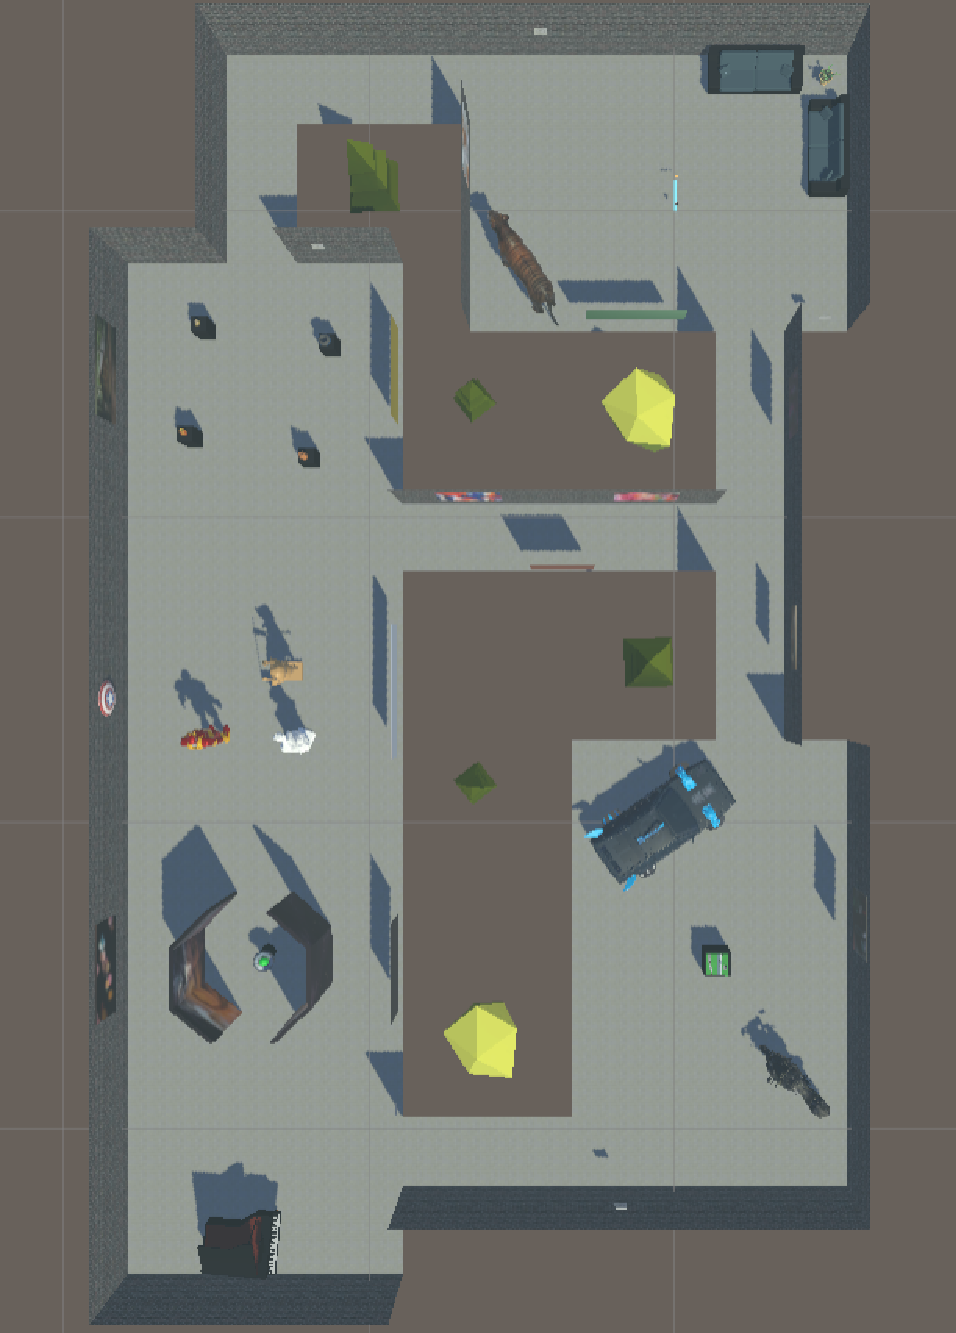
\includegraphics[width=0.25\textwidth]{images/museum-2-objects.pdf}
	\caption{The virtual rooms used for the study with a (1) Tutorial room, (2) Room A and (3) Room B.}
	\label{fig:study-environment}
\end{figure}

\subsection{Study Plan}
\label{subsection DPUS SP: Study Plan}
We explained the study setup in \cref{subsection DPUS SP: Study Setup} and now we will see the study plan. Before the study was even conducted participants were emailed with the details of the study and asked for consent to be sent over email. Due to the Covid-19 pandemic, certain precautions had to be given in the email as well. The exact draft of the email can be found in the appendix. Once the participants arrived the study could begin in the order shown in \cref{fig:study-plan}. The steps shown in this diagram will be explained further in this section. Before and after the study all hardware and stationary that the participant would use was sanitized in accordance with Covid-19 hygiene guidelines. The experimenter also wore a mask during the study.

\begin{figure}[]
	\centering
	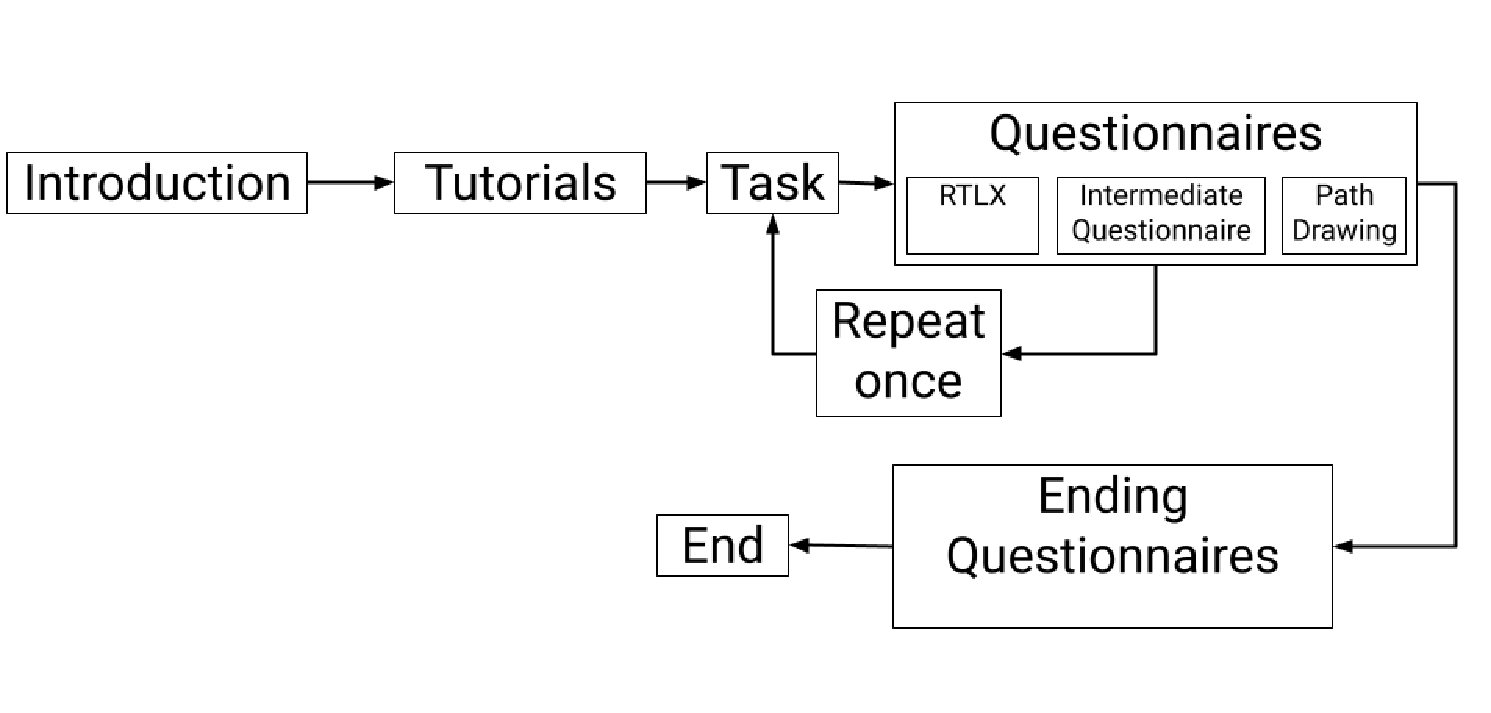
\includegraphics[width=0.8\textwidth]{images/study-plan.pdf}
	\caption{The study steps. Participants undergo one round of tests for each study condition. The study order was alternated between participants.}
	\label{fig:study-plan}
\end{figure}

\subsubsection{Tutorial and Tasks}
\label{subsubsection DPUS SP SP: Tutorial and Tasks}
When participants arrived they were seated in the chair where they would remain for the duration of the study. Then they were once again reminded of what they are consenting to before beginning an audio and screen recording. Participants were also reminded that they could stop the study at any time. They were then given a short briefing on the study process and told that they would begin with a tutorial on two techniques and then carry out two tasks with a questionnaire in between and at the end of these tasks. They also entered some demographic information to the questionnaire before beginning.

Before wearing the headset participants were shown the hand gestures that would need to be used as well as the button on the controller that they would need. The hand gestures were called name thumbs up, hand up and pointing. The controller button used would be the trigger button on the right hand controller. Pressing down on the button would give the feedback to allow the user to choose where to jump. Rotating the hand around the wrist would allow participants to control the orientation they would be at after the jump while moving the hand forward and back would influence the position. Once the position and orientation are selected the trigger button can be release to make the jump. Gestures and button mapping are shown in \cref{fig:gestures-controller}. Then the user could wear the Oculus Quest 2 and begin with the study tasks. The study started with a tutorial that was divided in two parts for the two techniques with the order they were presented in depending on the study order that they would be following. There were two possible study orders that could be followed. Automated guiding in the first task and free jumping in the second or vice versa. The tutorials would also be presented in this order. The study orders were alternated between participants. The participants could repeat the tutorials for each technique till they were comfortable with it. The time taken for each tutorial was also recorded. 

\begin{figure}[]
	(\centering 1)
	
\includegraphics[width=0.2\textwidth]{images/thumbs-up.pdf}
	(\centering 2)
	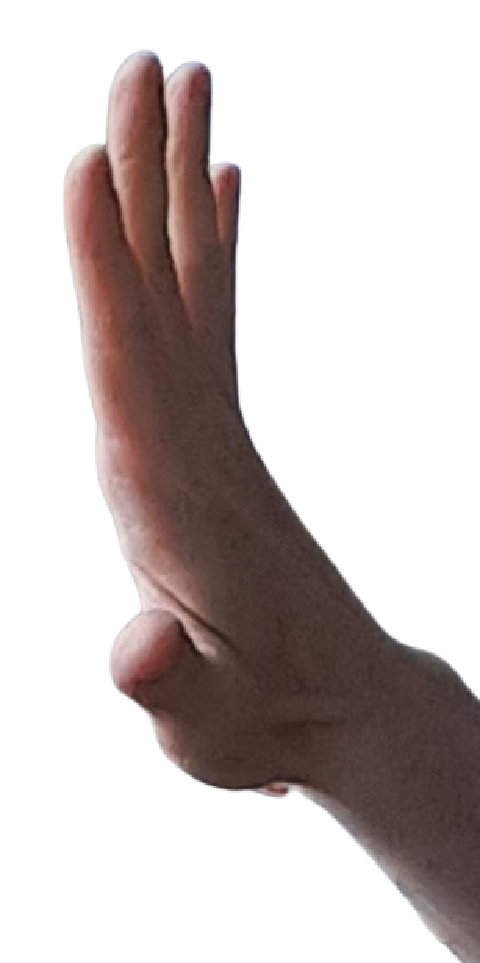
\includegraphics[width=0.2\textwidth]{images/hand-up.pdf}
	(\centering 3)
	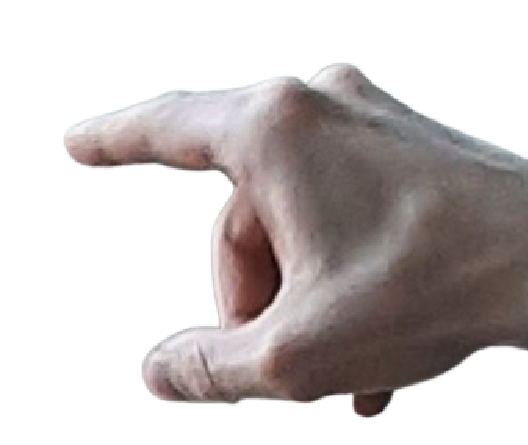
\includegraphics[width=0.2\textwidth]{images/pointing.pdf}
	(\centering 3)
	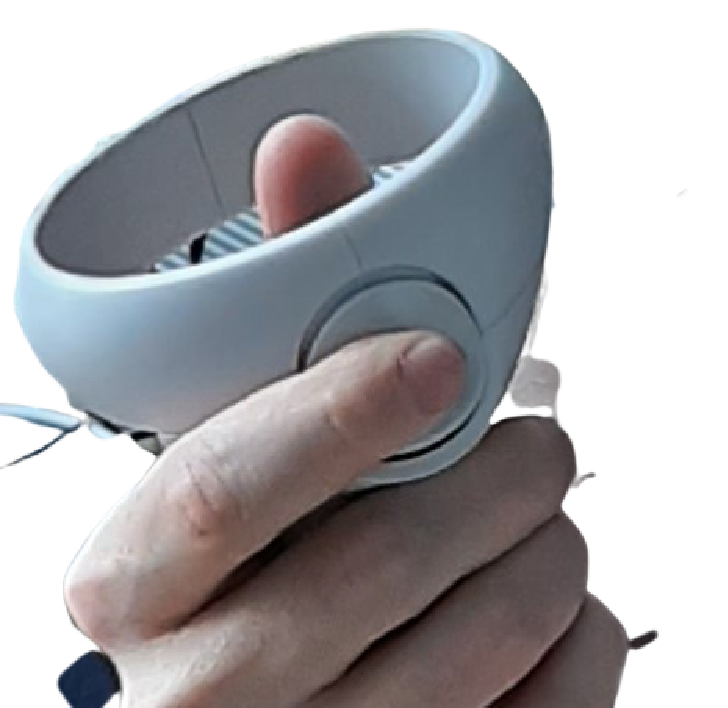
\includegraphics[width=0.2\textwidth]{images/controller.pdf}
	\caption{The gestures: (1) Thumbs Up to resume, (2) Hand Up to pause and (3) Pointing to choose between nodes for the Automated Guided Jumping technique. (4) The right controller trigger button that has to be pressed and released to make a jump in the Free Jumping condition.}
	\label{fig:gestures-controller}
\end{figure}

Once participants completed both the tutorials they could begin with the tasks. Each task was the same except for the technique and environment. Participants were told to use the technique to move through the environment. They could pause when necessary and look around at objects. When presented with a choice between 2 nodes they could pick whichever node they wanted. They were informed that they would need to draw their path and what they saw and therefore they should try and pay attention to where they were going. As participants moved through the environment their time, positions and orientations were recorded into a log file on every move and any time they paused or had to make a choice. When they chose a node the selected node was also logged. Example logging data is shown in the appendix to demonstrate the format.

\subsubsection{Questionnaire}
\label{subsubsection DPUS SP SP: User Feedback}
In between tasks participants could take off their headset and go to the second computer to answer some questions and draw their path. The questions for each task were the same. Finally at the end of the study participants answered some final study questions about both techniques. The exact questions in the questionnaire can be seen in the appendix.

The demographic questions obtained from the questionnaire were age and gender. The intermediate questions used for the study included a question on simulator sickness which was introduced by Fernandes et al. to give a discomfort score~\cite{Fernandes2016}. Then the participants were also asked their perceived level of comfort and their reasons.

To measure the task load we decided to use an electronic version of the \acrfull{rtlx} questionnaire as introduced by Hart et al. as a method for mental workload assessment~\cite{Hart1988}~\cite{Hart2006}. We then had some questions about the technique used to get information regarding the comprehensibility of jumps. The questions were both quantitative and qualitative to get a clear understanding on what the participants understood about the technique and whether they were confused at any point about their position and orientation. After the task questions were answered participants had to draw the objects they saw and their paths on a provided map, which was a top down view of the room without any objects in it. This map can be seen in the appendix. This would then be compared with the actual environment for accuracy and given a \acrfull{prs} based on the \cref{eq:eq1} where \textbf{INW} stands for number of correctly identified nodes and way-points, \textbf{INW} stands for total number of nodes and way-points the participant saw including the ones they had to choose from but did not, \textbf{IEP} is the number of correctly identified exhibits and painting and \textbf{TEP} is the total number of exhibits and paintings. These ratios are multiplied by hundred to get them as a percentage and then divided by two to get the average. This means that the range of possible path recall scores is from 0 to 100. Nodes and way-points are considered \textbf{INW} if they are drawn withing a circle of 1 centimeter radius around the actual position to account for human errors when remembering relative positions. This 1 centimeter on paper is equivalent to 2 meters on the unity environment. Paintings and exhibits that are drawn by participants on the map are considered \textbf{IEP} in the same way. 
\begin{equation}
	\label{eq:eq1}
	PRS = \frac{100\left(\frac{INW}{TNW} + \frac{IEP}{TEP}\right)}{2}
\end{equation}

Finally, after participants answered questions for Task B there were some final study questions to get quantitative feedback on the participants preferred technique and the reasons for it, as well as additional feedback on what they liked about each technique, what situations they would prefer it in and any other feedback about the techniques. This allowed us to have a more holistic view of the experience the users had with each technique.





%%%%%%%
% Evaluation of the User Study
%%%%%%%

\chapter{Evaluation of the User Study}
\pagenumbering{arabic}
\label{Chapter:Evaluation of the User Study}


%%%%%%%
% Conclusion and Future Work
%%%%%%%

\chapter{Conclusion and Future Work}
\pagenumbering{arabic}
\label{Chapter:Conclusion and Future Work}
In this thesis we looked into the need for a guided jumping navigation technique for immersive virtual environments.

We started with a look at related work in navigation and guiding for navigation. We looked into three travel metaphors, steering, teleportation and jumping. This led to a decision to focus on the jumping metaphor as it balances a good spatial understanding with reduced simulator sickness for a majority of users. We also looked into guiding navigation techniques that included techniques with automatic guiding using steering navigation and a free guiding with exploration assistance. We decided to focus on an automatic guiding technique using jumping navigation and compare it with a technique using free jumping with visual guidance. The only difference between these techniques would be the level of user control to jump. We decided on developing an automated guided jumping technique because wanted a technique that would provide users with the ability to navigate a completely new environment with a pre-existing narrative structure without the need for tour guides to guide them through the environment. We also wanted the interface to be novice friendly and allow users to focus on the environment rather than the navigation technique. Finally, we wanted the technique to allow users to get relevant knowledge of the environment and avoid simulator sickness or any other kind of discomfort. We also noted that the such an automated guided jumping technique could be quite useful in environments where a narrative structure is important such as for virtual tours or storytelling in \acrshort{vr}.

After a look at the literature review and motivation we looked into the design and development of the automated guided jumping technique. The technique was developed such that the user would be automatically jumping from one node or way point to another. Nodes in this case are points of interest while way points are points in between the nodes to break the navigation from one node to the next into smaller distances such that it could be called a jump and users would not miss anything. To ensure users were not surprised by the jumps we also designed and developed visual feedback about the jump including avatars at the next position and orientation, a visual countdown before a jump and signs for pausing and making a choice. Finally, to allow users to have some control over pausing, resuming and making a choice we implemented simple hand gestures that users could use.

To explore the benefits of our technique we decided to conduct a study comparing it with a technique that would allow users to jump freely instead of being automatically guided. This free jumping technique would also have visual guidance that would be the same as the visual feedback given to the users in our automated guiding technique. The study comparing these techniques was conducted using 9 participants. The results from this study show

%%%%%%%
% Biblography
%%%%%%%

{\footnotesize
\bibliography{vr-thesis-template}{}
\bibliographystyle{ieeetr}
}

%%%%%%%
% Appendix
%%%%%%%

\appendix
\chapter{Appendix}
\label{Appendix}
This is the appendix...



\end{document}